%%***********************************************
%% Plantilla para TFM.
%% Escuela Técnica Superior de Ingenieros Informáticos. UPM.
%%***********************************************

%%-----------------------------------------------
%% Importar Preámbulo:
% -*-coding: utf-8 -*-
%%***********************************************
%% Plantilla para TFG.
%% Escuela Técnica Superior de Ingenieros Informáticos. UPM.
%%***********************************************
%% Preámbulo del documento.
%%***********************************************
\documentclass[a4paper,11pt]{book}
\usepackage[utf8]{inputenc}
\usepackage[T1]{fontenc}
\usepackage[english,spanish,es-lcroman]{babel}
\usepackage{bookman}
\decimalpoint
\usepackage{graphicx}
\usepackage{amsfonts,amsgen,amsmath,amssymb}
\usepackage[top=3cm, bottom=3cm, right=2.54cm, left=2.54cm]{geometry}
\usepackage{afterpage}
\usepackage{colortbl,longtable}
\usepackage[pdfborder={0 0 0}]{hyperref} 
\usepackage{pdfpages}
\usepackage{url}
\usepackage[stable]{footmisc}
\usepackage{parskip} % para separar párrafos con espacio.
\usepackage{hyperref}

\usepackage[
backend=bibtex,
style=ieee]{biblatex}       %use the biblatex package
%%-----------------------------------------------
\usepackage{fancyhdr}
\pagestyle{fancy}
\fancyhf{}
\fancyhead[LO]{\leftmark}
\fancyhead[RE]{\rightmark}
\setlength{\headheight}{1.5\headheight}
\cfoot{\thepage}

\addto\captionsspanish{ \renewcommand{\contentsname}
  {Tabla de contenidos} }
\setcounter{tocdepth}{4}
\setcounter{secnumdepth}{4}

\renewcommand{\chaptermark}[1]{\markboth{\textbf{#1}}{}}
\renewcommand{\sectionmark}[1]{\markright{\textbf{\thesection. #1}}}
\newcommand{\HRule}{\rule{\linewidth}{0.5mm}}
\newcommand{\bigrule}{\titlerule[0.5mm]}

\usepackage{appendix}
\renewcommand{\appendixname}{Anexos}
\renewcommand{\appendixtocname}{Anexos}
%\renewcommand{\appendixpagename}{Anexos}
%%-----------------------------------------------
%% Páginas en blanco sin cabecera:
%%-----------------------------------------------
\usepackage{dcolumn}
\newcolumntype{.}{D{.}{\esperiod}{-1}}
\makeatletter
\addto\shorthandsspanish{\let\esperiod\es@period@code}

\def\clearpage{
  \ifvmode
    \ifnum \@dbltopnum =\m@ne
      \ifdim \pagetotal <\topskip
        \hbox{}
      \fi
    \fi
  \fi
  \newpage
  \thispagestyle{empty}
  \write\m@ne{}
  \vbox{}
  \penalty -\@Mi
}
\makeatother
%%-----------------------------------------------
%% Estilos código de lenguajes: Consola, C, C++ y Python
%%-----------------------------------------------
\usepackage{color}

\definecolor{gray97}{gray}{.97}
\definecolor{gray75}{gray}{.75}
\definecolor{gray45}{gray}{.45}

\usepackage{listings}
\lstset{ frame=Ltb,
     framerule=0pt,
     aboveskip=0.5cm,
     framextopmargin=3pt,
     framexbottommargin=3pt,
     framexleftmargin=0.4cm,
     framesep=0pt,
     rulesep=.4pt,
     backgroundcolor=\color{gray97},
     rulesepcolor=\color{black},
     %
     stringstyle=\ttfamily,
     showstringspaces = false,
     basicstyle=\scriptsize\ttfamily,
     commentstyle=\color{gray45},
     keywordstyle=\bfseries,
     %
     numbers=left,
     numbersep=6pt,
     numberstyle=\tiny,
     numberfirstline = false,
     breaklines=true,
   }
\lstnewenvironment{listing}[1][]
   {\lstset{#1}\pagebreak[0]}{\pagebreak[0]}

\lstdefinestyle{consola}
   {basicstyle=\scriptsize\bf\ttfamily,
    backgroundcolor=\color{gray75},    
    }

\lstdefinestyle{CodigoC}
   {basicstyle=\scriptsize,
	frame=single,
	language=C,
	numbers=left
   }
   
\lstdefinestyle{CodigoC++}
   {basicstyle=\small,
	frame=single,
	backgroundcolor=\color{gray75},
	language=C++,
	numbers=left
   }

\lstdefinestyle{Python}
   {language=Python,    
   }
\makeatother   
\addbibresource{secciones/08_Bibliografia.bib} 
%%-----------------------------------------------
%% Cargar datos relativos al TFM:
%% (actualizar estos datos en secciones/_DatosTFM.tex) 
%%***********************************************
%% Plantilla para TFM.
%% Escuela Técnica Superior de Ingenieros Informáticos. UPM.
%%***********************************************
%% Información requerida para completar la portada.
%%*********************************************** 

%% Escribe Nombre y Apellidos del autor del trabajo:
\newcommand{\NombreAutor}{Luna Jiménez Fernández}

%% Escribe el Grado: 
\newcommand{\Master}{Inteligencia Artificial}

%% Escribe el Título del Trabajo:
\newcommand{\TituloTFM}{ Navegación Reactiva Aplicada a Agentes Fisicos en Entornos Domésticos usando Habitat Sim } 

%% Escribe Nombre y Apellidos del Tutor del trabajo: 
\newcommand{\NombreTutor}{Martín Molina Gómez} 
\newcommand{\NombreCoTutor}{María Julia Flores Gallego} 

% Escribe el Departamento al que pertenece el Tutor:
\newcommand{\Departamento}{Computer Vision and Aerial Robotics (CVAR)}

% Escribe la fecha de lectura, en formato: Mes - Año
\newcommand{\Fecha}{Septiembre - 2021}
%%***********************************************


%%-----------------------------------------------
%% Documento:
\begin{document}
%%***********************************************
%% Plantilla para TFM.
%% Escuela Técnica Superior de Ingenieros Informáticos. UPM.
%%***********************************************
%% Portada. 
%%***********************************************
\begin{titlepage}

\begin{minipage}{0.15\linewidth}
\hspace*{-2.5cm}
\noindent

\includegraphics[scale=0.5]{./imagenes/EscUpm.png} \qquad\qquad
\end{minipage}
\begin{minipage}{0.7\linewidth}
\begin{center}
\huge{ Universidad Politécnica\\de Madrid }\\
\vspace*{0.5cm}
\Large{\textbf{Escuela Técnica Superior de \\
Ingenieros Informáticos}}
\end{center}
\end{minipage}
\begin{minipage}{0.2\linewidth}

\includegraphics[scale=0.5]{./imagenes/FacInformatica.png} 
\end{minipage}

\vspace*{1cm}
\begin{center}
\Large{Máster Universitario en  \Master{} }
\end{center}

\vspace*{1cm}
\begin{center}
\huge{ Trabajo Fin de Máster }
\end{center}

\vspace*{0.5cm}
\begin{center}
\huge\bfseries {  \TituloTFM{} } 
\end{center}

\vspace*{5cm}

\noindent
\large{Autor(a): \NombreAutor{} }\\
\large{Tutor(a): \NombreTutor{} }


\vspace*{4cm}
\begin{center}
Madrid, \Fecha
\end{center}

%%--------------------------------
\newpage
\thispagestyle{empty}
%%--------------------------------
\noindent
Este Trabajo Fin de Máster se ha depositado en la ETSI Informáticos de la Universidad Politécnica de Madrid para su defensa.

\vspace*{4cm}
\noindent
\textit{Trabajo Fin de Máster}\\
\textit{Máster Universitario en} \Master{}

\begin{enumerate}
\item[\textit{Título:}] \TituloTFM{}
\end{enumerate}
\Fecha


\vspace*{3cm}

\noindent
\begin{tabular}{ll}
\textit{Autor(a):} & \NombreAutor{}  \\ 
\textit{Tutor(a):} & \NombreTutor{}  \\ 
                & \Departamento{} \\
                & ETSI Informáticos\\
                & Universidad Politécnica de Madrid
\end{tabular} 

\end{titlepage}


%%-----------------------------------------------
%% Numeración romana:
\frontmatter
%%-----------------------------------------------
\chapter*{Resumen}

<<Aquí va el resumen del TFM. Extensión máxima 2 páginas.>>

%%--------------
\newpage
%%--------------

\chapter*{Abstract}

<<Abstract of the Master Project. Maximum length: 2 pages.>>


%%%%%%%%%%%%%%%%%%%%%%%%%%%%%%%%%%%%%%%%%%%%%%%%%%%%%%%%%%%
%% Final del resumen. 
%%%%%%%%%%%%%%%%%%%%%%%%%%%%%%%%%%%%%%%%%%%%%%%%%%%%%%%%%%%

\chapter*{Agradecimientos}

\tableofcontents

\listoffigures

%%-----------------------------------------------
%% Numeración arábiga:
\mainmatter
%%----------------------------------------------- 
\chapter{Introducción}

En este capítulo se realizará una breve introducción a los contenidos que serán expuestos posteriormente a lo largo de la memoria. Tras ésta presentación, se expondrá la motivación que ha propiciado el desarrollo de este trabajo. Finalmente, se describirá la estructura seguida por la memoria.

\section{Introducción}
LO TIPICO DE INTRO

\section{Motivación}
LO TIPICO DE MOTIVACION

\section{Estructura}


Esta memoria está dividida en un total de 7 capítulos, que serán descritos brevemente a continuación.

\begin{itemize}
	\item \textbf{Capítulo 1:} En este capítulo se introduce el trabajo desarrollado, la motivación que ha llevado a éste y la estructura general de la memoria.
	\item \textbf{Capítulo 2:} En este capítulo se describe en profundidad el problema a resolver, presentando los antecedentes previos al trabajo realizado y detallando los objetivos que se esperan cumplir.
	\item \textbf{Capítulo 3:} En este capítulo se realiza una revisión de las principales técnicas en los campos relacionados con el trabajo: \textit{deep learning} y redes neuronales convolucionales, aprendizaje por refuerzo (estudiando tanto las técnicas clásicas como las técnicas de aprendizaje por refuerzo profundo) y algunos de los principales algoritmos de navegación automática.
	\item \textbf{Capítulo 4:} En este capítulo se presentan tanto \textit{Habitat Sim} como \textit{Habitat Lab}, las principales herramientas usadas durante el desarrollo del trabajo. De estas herramientas se comenta además su instalación y sus dependencias. Finalmente, se exponen los principales conceptos de Habitat Lab, explicando su funcionamiento y dando detalles de la implementación propia realizada.
	\item \textbf{Capítulo 5:} En este capítulo se detalla el diseño del agente de navegación reactiva propuesto. Se describe tanto la representación del conocimiento (estado, acciones y recompensas) como la arquitectura, el método de actuación y el entrenamiento llevado a cabo por el agente. Finalmente, se realiza una breve explicación del funcionamiento y la arquitectura del resto de agentes usados como \textit{benchmarks} y comparativas ofrecidos por \textit{Habitat Lab}.
	\item \textbf{Capítulo 6:} En este capítulo se detalla la experimentación realizada, indicando los parametros utilizados. Además, se presentan los resultados y el rendimiento obtenido por los agentes tanto durante el entrenamiento como durante la evaluación posterior.
	\item \textbf{Capítulo 7:} Finalmente, en este capítulo se presentan las conclusiones alcanzadas tras el desarrollo del trabajo, proponiendo posibles lineas de trabajo futuro para continuarlo.
\end{itemize}

Además, al final de la memoria se incluye una bibliografía en la que se encuentra la lista de fuentes y referencias usadas a lo largo de ésta.

%%---------------------------------------------------------

\chapter{Descripción del problema}

En este capítulo se planteará en detalle el problema a resolver. Tras esto, se comentarán soluciones previas propuestas al problema, y se describirán los objetivos que se esperan alcanzar con el desarrollo del trabajo. 

\section{Definición del problema}

El problema a resolver es el diseño de un agente físico (un robot) capaz de navegar desde una posición inicial hasta una posición final (conocidas sus coordenadas) en un entorno de interior del que no se tiene conocimiento previo (como puede ser el interior de una casa) de forma eficiente. Este problema se encuadra en el campo de la navegación automática, concretamente en el de la \textbf{navegación a meta} (\textit{Point Goal Navigation}) \textbf{sin exploración previa} del entorno \cite{DBLP:journals/corr/abs-1807-06757}.

Para lograr esto, es necesario entrenar al agente en un entorno controlado para que aprenda a navegar de forma autónoma en interiores desconocidos, usando alguna técnica de aprendizaje por refuerzo. Además. se busca que el agente sea capaz de navegar \textbf{sin exploración previa} (como se ha mencionado anteriormente), buscando un sistema reactivo frente a uno basado en exploración-navegación.

El agente físico cuenta con las siguientes características a tener en cuenta:
\begin{itemize}
	\item \textbf{Movimiento:} El agente es terrestre (se desplaza con ruedas sobre el suelo), pudiendo moverse hacia adelante y rotar sobre si mismo. El agente no es capaz de realizar movimientos ortogonales.
	\item \textbf{Sensores:} El agente cuenta con dos sensores para recibir información del entorno: una \textbf{cámara de profundidad} para observar el espacio frente al robot y un \textbf{GPS}, indicando la distancia y ángulo hasta la meta.
\end{itemize}

\section{Antecedentes}

La navegación autónoma de robots en interiores es un campo de gran interés tanto para la investigación como para la industria, existiendo gran cantidad de grupos dedicados a la propuesta y desarrollo de agentes capaces de resolver estos problemas de forma eficaz.

Algunos ejemplos de este interés \textit{Habitat Challenge}, un desafío anual organizado por  \textit{Facebook AI Research} (el grupo de investigación de inteligencia artificial de Facebook) parte de la \textit{Conference on Computer Vision and Pattern Recognition (CVPR)} en el que se buscan los mejores algoritmos para resolver problemas de \textbf{navegación autónoma a metas} \cite{habitat2020sim2real} (aunque también incluye problemas de \textbf{navegación autónoma a objetos} \cite{batra2020objectnav}) aplicados a agentes físicos en entornos de interiores. Algunas de las mejores propuestas de estos últimos años han sido:
 
\begin{itemize}
	\item \textbf{Devendra Singh Chaplot \textit{et al.} (2019)} \cite{DBLP:journals/corr/abs-2004-05155}: Se propone un nuevo algoritmo, \textit{Active Neural SLAM}, que combina las capacidades de planificadores de ruta clásicos como SLAM con la capacidad del aprendizaje por refuerzo profundo para generar políticas de acciones locales y globales. Esta propuesta obtuvo el primer puesto del \textit{Habitat Challenge 2019}.
	\item \textbf{Santhosh K. Ramakrishnan \textit{et al.} (2020)} \cite{DBLP:journals/corr/abs-2008-09285}: Se propone un sistema de navegación entrenado con aprendizaje por refuerzo que, a partir de sus observaciones a través de una cámara RGB, es capaz de inferir la posición de los objetos más allá de su ángulo de visión para mejorar su rendimiento a la hora de generar un mapa de su entorno. Esta propuesta alcanzó el primer puesto del \textit{Habitat Challenge 2020}.
	 \item \textbf{Samyak Datta \textit{et al.} (2020)} \cite{DBLP:journals/corr/abs-2009-03231}: Se propone un sistema de navegación entrenado con aprendizaje por refuerzo (\textit{PPO}) que tiene en cuenta el ruido existente en entornos reales (problemas durante la actuación, desviaciones entre la posición real y estimada...) haciendo esfuerzo para corregirlo. Esta propuesta alcanzó el segundo puesto del \textit{Habitat Challenge 2020}.
	 \item \textbf{Ruslan Partsey (2021)} \cite{Partsey2021}: Se desarrolla un agente que usa técnicas de odometría (usar datos de sensores de movimiento para estimar la posición real) visual con aprendizaje por refuerzo para conseguir una navegación eficiente en entornos con ruido. Esta propuesta alcanzó el primer puesto del \textit{Habitat Challenge 2021}.
\end{itemize}

Si bien todas las propuestas anteriores utilizan técnicas de aprendizaje por refuerzo, la gran mayoría de éstas utilizan enfoques basados en el mapeado y navegación de los entornos, frente a una propuesta puramente reactiva (sin mapa) como la de éste trabajo.

El antecedente más directo al trabajo descrito en esta memoria es la propuesta realizada por \textbf{Carlos Sampedro \textit{et al.} (2018)} \cite{Sampedro2018}, siendo éste trabajo una adaptación y continuación directa. El agente propuesto utiliza un método basado en campos de potenciales, entrenado con aprendizaje por refuerzo profundo para navegar un dron aéreo a través de entornos de interior, usando un conjunto de láseres (para percibir el entorno a su alrededor) y la posición relativa del propio dron respecto a la meta, con buenos resultados. Esta arquitectura se puede observar en la Figura \ref{fig:chap2-drone}.

\begin{figure}[h]
    \centering
    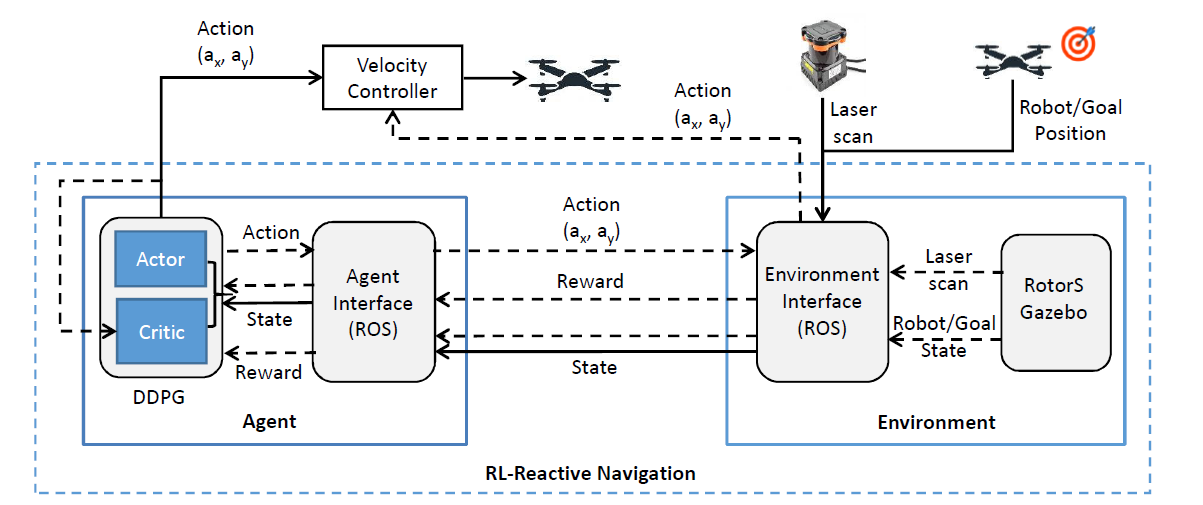
\includegraphics[width=\textwidth]{imagenes/cap2/drone-architecture.png}
    \caption{Arquitectura propuesta para el sistema de navegación reactivo original \cite{Sampedro2018}.}
    \label{fig:chap2-drone}
\end{figure}

Ahora bien, existen diferencias destacables entre la propuesta original y el trabajo descrito en esta memoria:

\begin{itemize}
	\item \textbf{Movimientos del agente:} La propuesta original utiliza como agente a un dron multirotor, capaz de navegar por el aire (aunque se mantiene a una altura constante) y de realizar movimiento omnidireccional. En cambio, el trabajo desarrollado utiliza un robot terrestre (susceptible a obstáculos en el suelo) incapaz de movimiento omnidireccional, siendo necesario el giro del agente para poder esquivar obstáculos y desplazarse.
	\item \textbf{Sensores del agente:} Mientras que la propuesta original utiliza un conjunto de láseres para percibir su entorno, el trabajo desarrollado propone un agente con una única cámara de profundidad frontal. Si bien el conjunto de láseres resulta más caro que una cámara de profundidad, también ofrece un ángulo de visión mayor de los obstáculos del entorno.
	\item \textbf{Complejidad del entorno:} La propuesta original entrena al agente en entornos de interior simples (contando con espacios simples con obstáculos dispersos), frente a los entornos usados por el trabajo desarrollado (siendo recreaciones del interior de domicilios, incluyendo topografías más complejas con cuartos y una mayor cantidad de obstáculos y ruido).
\end{itemize}

\section{Objetivos}

El principal objetivo de este trabajo es el estudio y aplicación de técnicas de aprendizaje por refuerzo profundo y navegación autónoma basada en campos de potenciales para el desarrollo de un agente capaz de navegar entornos de interior, evaluando su viabilidad y eficacia.

Para cumplir este objetivo, es necesario a su vez cumplir una serie de objetivos parciales:

\begin{itemize}
	\item Revisión de bibliografía para comprender plenamente las técnicas a usar durante el desarrollo.
	\item Búsqueda y evaluación de librerías y herramientas disponibles para el desarrollo del agente (incluyendo simuladores, entornos de trabajo...)
	\item Caracterización, formalización e implementación del agente y de posibles variaciones propuestas dentro del entorno elegido, para poder ser evaluado posteriormente.
	\item Realización de experimentos para estudiar el comportamiento del agente durante el entrenamiento y posteriormente al enfrentarse a problemas reales.
	\item Estudio y análisis de los resultados, realizando comparación con \textit{benchmarks} para extraer observaciones y conclusiones que permitan valorar la viabilidad y eficacia del agente propuesto.
\end{itemize}

Este trabajo además aborda un segundo objetivo, el estudio y uso del simulador \textit{Habitat Sim}, con el fin de evaluar su utilidad de cara a posteriores trabajos. Para esto, se plantean los siguientes objetivos parciales:

\begin{itemize}
	\item Revisión y estudio de documentación oficial y ejemplos ofrecidos por el simulador.
	\item Desarrollo del agente descrito previamente en el marco del simulador, usando las herramientas ofrecidas.
	\item Creación de documentación sobre el uso adecuado del simulador para facilitar trabajos posteriores.
	\item Evaluación de la idoneidad del simulador para la resolución de problemas de navegación autónoma.
\end{itemize}

\chapter{Revisión de técnicas}

\section{\textit{Deep Learning}}
[SOBRE DEEP LEARNING, REDES NEURONALES PROFUNDAS Y CNNs]

\section{Aprendizaje por refuerzo}
[APRENDIZAJE POR REFUERZO, Q LEARNING (y quizas otros clasicos?), DEEP Q LEARNING (y mejoras), AGENTE / CRITICO, PPO...]

[SECCIONES TENTATIVAS]
\subsection{Algoritmos de aprendizaje por refuerzo clásicos}

\subsection{Algoritmos de aprendizaje por refuerzo profundos}


\section{Algoritmos de navegación automática}
[DE ESTO SE MENOS, ASI QUE PUEDO PREDECIR MENOS]


\chapter{\textit{Habitat}: Simulador \textit{Habitat Sim} y \textit{Habitat Lab}}

En este capítulo se describirá en profundidad el simulador utilizado, \textit{Habitat Sim 2.0}, y su librería de Python \textit{Habitat Lab}. Además, se presentarán los principales componentes usados por la librería, detallando su funcionamiento y su uso. Finalmente, se explicará la instalación del simulador y las dependencias necesarias.

\section{\textit{Habitat}}

\textbf{\textit{Habitat}} \cite{habitat19iccv} es una plataforma para el desarrollo de inteligencia artificial con agentes físicos, diseñada con el fin de estandarizar el conjunto de herramientas necesarias para el entrenamiento en entornos hiperrealistas tridimensionales bajo una sola plataforma unificada e integrada.

Esta plataforma pretende resolver algunos de los problemas tradicionales que afectan a otros simuladores, impidiendo la generalización y comparación de resultados experimentales \cite{habitat19iccv}:
\begin{itemize}
	\item La dependencia entre componentes (como simuladores funcionando únicamente con conjuntos de datos o tareas especificas), dificultando el trabajo al necesitar varias herramientas.
	\item Los parámetros fijos (como las acciones disponibles, los sensores...), dificultando la comparativa de resultados.
	\item El rendimiento subóptimo de los simuladores (tanto en renderizado como en físicas), dificultando el entrenamiento de agentes a gran escala. 
\end{itemize}

La plataforma \textit{Habitat} cuenta con dos componentes principales \cite{habitat19iccv}:
\begin{itemize}
	\item \textbf{\textit{Habitat Sim}:} Un simulador 3D modificable con agentes configurables, diversos sensores y manejo de conjuntos de datos 3D genéricos (con soporte de fábrica para conjuntos como \textit{Matterport3D} o \textit{Gibson}).
	\item \textbf{\textit{Habitat Lab}:} Una librería modular de alto nivel desarrollada para Python, con el fin de facilitar el desarrollo de agentes físicos en \textit{Habitat Sim}, ofreciendo herramientas para la definición, configuración, entrenamiento y evaluación de éstos.
\end{itemize}

\subsection{Simulador \textit{Habitat Sim}}

\textbf{\textit{Habitat Sim}} \cite{habitat19iccv} es un simulador 3D ampliable, diseñado para el entrenamiento de agentes físicos en entornos hiperrealistas. Este simulador se encarga de representar escenarios tridimensionales en formatos estandarizados y de simular agentes físicos, tanto sensores como movimiento. 

Este simulador fue diseñado con el propósito de solventar los problemas descritos previamente, siendo algunos de sus objetivos principales:

\begin{itemize}
	\item \textbf{Soporte genérico a conjuntos de datos:} \textit{Habitat Sim} es capaz de reconstruir y simular conjuntos de datos genéricos independientemente de su origen, usando un formato uniforme y estandarizado como son los \textit{scene graphs} \cite{DBLP:journals/corr/abs-2104-01111} (representaciones estructuradas de los escenarios). Esta estandarización permite al simulador trabajar de forma consistente con cualquier conjunto de datos.
	\item \textbf{Modularidad:} El simulador está diseñado ofreciendo \textit{APIs} de todos sus componentes, permitiendo la ampliación del simulador con nuevos sensores, escenarios, tareas...
	\item \textbf{Rendimiento:} \textit{Habitat Sim} está implementado en C++ usando la librería \textit{Magnum Graphics} como \textit{middleware} para el procesamiento de la imagen. Además, la tubería de creación y renderizado de imágenes está optimizada para evitar la repetición de procesos, siendo capaz de generar todas las imágenes de cada instante en una única pasada.
	
	Todo ésto permite al simulador generar miles de \textit{frames} por segundo, siendo este valor al menos un orden de magnitud superior al que ofrecen otros simuladores como \textbf{Gibson} \cite{xiazamirhe2018gibsonenv} o \textbf{MINOS} \cite{DBLP:journals/corr/abs-1712-03931}. Esta velocidad mueve el cuello de botella de la simulación al entrenamiento del agente, permitiendo entrenamientos más profundos en menos tiempo.
\end{itemize}

\textbf{\textit{Habitat 2.0}} \cite{szot2021habitat} es una versión posterior de \textit{Habitat Sim} lanzada en Junio de 2021, diseñada con el fin de ser capaz de simular entornos interactivos con físicas complejas (frente a las simulaciones de físicas simples de \textit{Habitat Sim}) y centrada en permitir la creación y evaluación de agentes físicos asistentes. Las principales características ofrecidas son:

\begin{itemize}
	\item \textbf{Simulador \textit{Habitat 2.0}:} Una segunda versión del simulador \textit{Habitat Lab} con capacidad para simular movimientos y físicas de objetos rígidos (como puertas, cajones...), robots articulados, cinemáticas, dinámicas...
	
El rendimiento del simulador es superior al de \textit{Habitat Sim}, especialmente durante la simulación de físicas. Además, el rendimiento escala notablemente, pudiendo trabajar de forma distribuida. 
	
	\item \textbf{Conjunto de datos \textit{ReplicaCAD}:} \textit{ReplicaCAD} es un conjunto de datos creado a partir del conjunto \textit{Replica} \cite{DBLP:journals/corr/abs-1906-05797}. Este conjunto de datos está diseñado para aprovechar las capacidades del nuevo simulador y pensado para evaluación de tareas de reorganización de elementos, implementando objetos articulados e interactivos.
	
	\item \textbf{\textit{Home Assistant Benchmark (HAB)}:} Un \textit{benchmark} implementando un conjunto de tareas típicas para robots asistentes (como limpiar un cuarto o preparar una mesa), diseñado para evaluar el rendimiento de estos agentes de forma estandarizada.
\end{itemize}

\subsection{Librería \textit{Habitat Lab}}

\textit{Habitat Lab} (originalmente conocido como \textit{Habitat-API}) \cite{habitat19iccv} es una librería modular de alto nivel desarrollada para \textit{Python}, con el fin de facilitar el uso de \textit{Habitat Sim} y el desarrollo de agentes físicos. El principal objetivo de la librería es permitir a los usuarios:

\begin{itemize}
	\item \textbf{Definir tareas para agentes físicos}: Se ofrecen tareas típicas (como navegación, seguimiento de orden, búsqueda de objetos...) y \textit{APIs} para desarrollar tareas propias.
	\item \textbf{Configurar agentes físicos:} Se permite modificar al agente físico ajustando su forma  física, los sensores disponibles, las acciones posibles...
	\item \textbf{Entrenar agentes físicos:} Se ofrece soporte para técnicas clásicas (como \textit{SLAM}) además de entrenamiento por refuerzo y entrenamiento por imitación.
	\item \textbf{Evaluar agentes físicos:} Se ofrecen métricas estándares \cite{DBLP:journals/corr/abs-1807-06757} usadas para evaluar el rendimiento de los agentes.
\end{itemize}

Además, la librería opcionalmente ofrece \textit{Habitat Baselines}, un conjunto de ejemplos y ampliaciones a \textit{Habitat Lab}. Entre estas ampliaciones se incluyen diversas utilidades para facilitar el desarrollo, agentes prediseñados y ejemplos para entender el funcionamiento del simulador y la librería.


\section{Conceptos principales de \textit{Habitat}}

La arquitectura de \textit{Habitat} (y, especialmente, la de la librería \textit{Habitat Lab}) gira principalmente en torno a tres conceptos principales, como se puede ver en la Figura \ref{fig:chap4-habitat}:

\begin{figure}[h]
    \centering
    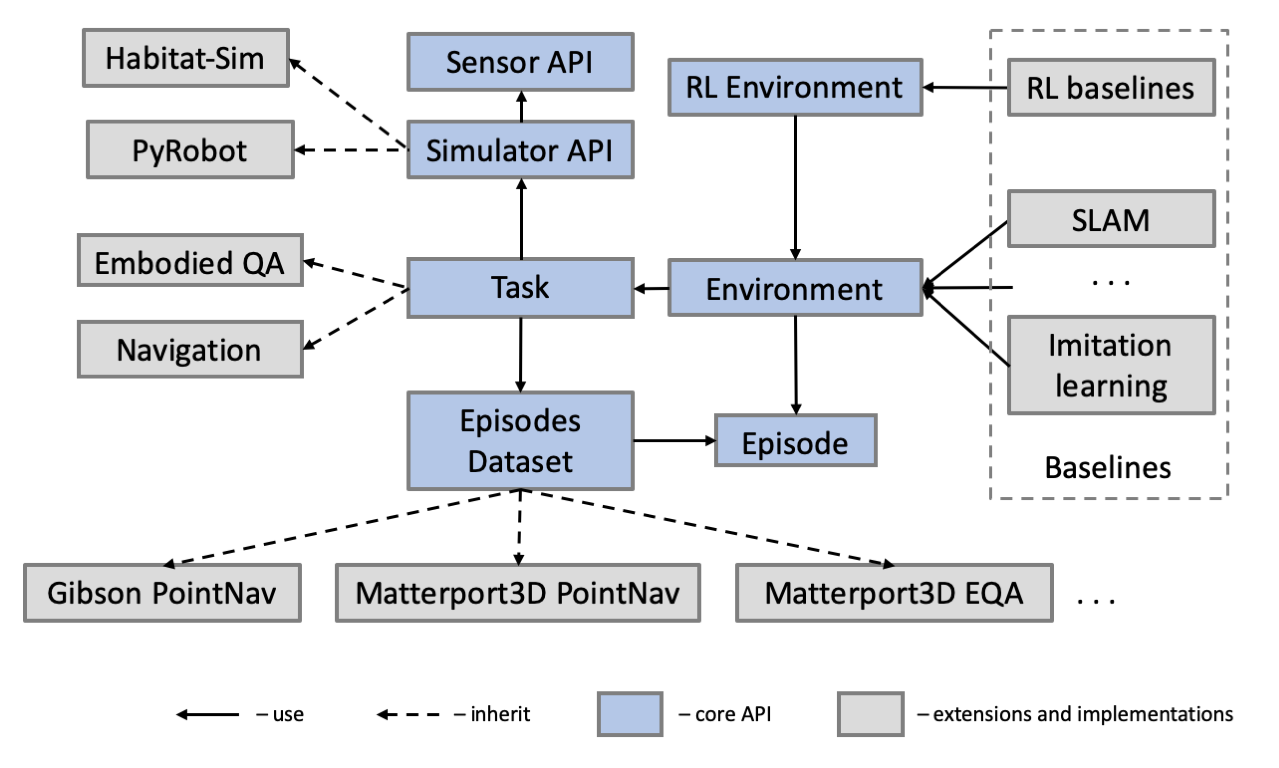
\includegraphics[width=\textwidth]{imagenes/cap4/habitat_lab_structure.png}
    \caption{Arquitectura de \textit{Habitat Lab} \cite{habitat19iccv}.}
    \label{fig:chap4-habitat}
\end{figure}

\begin{enumerate}
	\item \textbf{Tarea (\textit{Task)}:} El problema concreto a resolver por el agente, gestiona los objetivos y el éxito de la tarea usando métricas del simulador.
	\item \textbf{Episodio (\textit{Episode)}:} Especificación del episodio a realizar, conteniendo información como la posición y ángulo iniciales del agente, posición de la meta...
	\item \textbf{Entorno (\textit{Environment)}:} Concepto principal del simulador, abstrae toda la información necesaria para permitir el trabajo con el simulador y el agente físico.
\end{enumerate}

Ahora bien, la documentación oficial del simulador es pobre y ofrece poca información sobre los conceptos y, especialmente, sobre su uso. Además, hay otros conceptos (como entrenadores, ficheros de configuración...) de igual relevancia e importancia para el uso del simulador que no reciben ninguna explicación. 

Por tanto, en esta sección se busca explicar en detalle los conceptos principales necesarios para trabajar con \textit{Habitat}, detallando sus características y su uso.

\subsection{Entornos}

Un \textbf{entorno (\textit{environment})} es el concepto principal de \textit{Habitat Lab}. El entorno se encarga de abstraer las principales tareas necesarias para el trabajo con agentes físicos, siendo las principales tareas que realiza:

\begin{itemize}
	\item \textbf{Carga y manejo del conjunto de datos:} El entorno se encarga de la lectura y carga de los ficheros, y de la conversión de los escenarios al formato de \textit{scene graph}. 
	\item \textbf{Control de las métricas y los objetivos de la tarea:} El entorno se encarga de la interacción con el simulador para el control de los objetivos y las métricas de la tarea. Además, se encarga de detener los episodios cuando se cumplen los objetivos.
	\item \textbf{Generación y manejo de los episodios:} El entorno genera la lista de episodios a partir del conjunto de datos y de la tarea a realizar. Además, se encarga de ordenar los episodios de forma óptima (juntando los episodios que se realizan en un mismo escenario) para agilizar el proceso.
	\item \textbf{Control del agente físico:} El entorno interactúa con el simulador en ambos sentidos, leyendo los sensores del agente físico y devolviendole la acción realizada para simular los resultados.
\end{itemize}

Por defecto, \textit{Habitat Lab} ofrece dos tipos de entornos, a partir de los cuales se puede derivar cualquier entorno necesario.

\subsubsection{\textit{Env}}

\textbf{\textit{Env}} es el simulador básico ofrecido por \textit{Habitat}, usado principalmente para agentes sin aprendizaje y para la evaluación de agentes entrenados, implementando todas las características descritas previamente. El entorno ofrece dos métodos básicos, usados para controlar la simulación:

\begin{itemize}
	\item \textbf{reset():} Este método se encarga de preparar el entorno para el comienzo de un episodio, cargando el escenario y configurándolo para el episodio actual. Además, devuelve las primeras observaciones que recibe el agente con el sensor, para poder actuar a partir de ellas.
	\item \textbf{step(acción):} Dada una acción como argumento, el entorno aplica la acción al agente físico y devuelve las nuevas percepciones del agente a través de sus sensores.
\end{itemize}

Cualquier entorno personalizado que se quiera crear debe ser una subclase de \textit{Env} (al ofrecer toda la funcionalidad básica).

\subsubsection{\textit{RLEnv}}

\textbf{\textit{RLEnv}} es la principal subclase de \textit{Env} disponible, ofreciendo capacidades adicionales al entorno para permitir el entrenamiento usando aprendizaje por refuerzo. Además de los métodos anteriores, incluye varios más que deben ser implementados para su funcionamiento:

\begin{itemize}
	\item \textbf{get{\_}reward(observaciones):} A partir de las observaciones del agente, calcula una recompensa o penalización para éste. En general, el procesamiento de recompensas se implementa directamente en el entorno a través de este método.
	
	\item \textbf{get{\_}reward{\_}range():} Este método únicamente devuelve los límites de la recompensa (el rango $[min, max]$ en el que se encuentra).
	
	\item \textbf{get{\_}done(observaciones):} A partir de las observaciones del agente, calcula si el episodio ha acabado (ya sea de forma satisfactoria o fallida). En este método se implementan comprobaciones como colisiones u otras condiciones de parada.
	
	\item \textbf{get{\_}info(observaciones):} Devuelve información respecto al entorno a partir de la última observación. Es típico devolver información de sensores o métricas con este método. 
\end{itemize}

Por defecto, \textit{RLEnv} no implementa los métodos descritos previamente, por lo que es necesario realizar un entorno personalizado para el entrenamiento. Ahora bien, \textit{Habitat Baselines} ofrece \textit{NavRLEnv}, una implementación básica de entorno pensado para problemas de navegación a objetivo que sirve como punto de partida para otras implementaciones más complejas.

En este trabajo, se ha implementado un entorno personalizado (\textit{ReactiveNavigationEnv}) como subclase de \textit{NavRLEnv}, con definiciones propias de los métodos previos para usar el sistema de recompensas basado en potenciales propuesto (descrito en más detalle en el Capítulo 5).

\subsection{Tareas}

Una \textbf{tarea (\textit{embodied task})} es un contenedor de la información necesaria para que el simulador pueda definir y trabajar con una tarea. Concretamente, contiene información sobre:

\begin{itemize}
	\item El \textbf{espacio de acciones} disponible.
	\item Los \textbf{sensores} disponibles para el agente.
	\item Las \textbf{métricas} a utilizar para valorar al agente.
	\item El \textbf{simulador} sobre el que se va a trabajar.
\end{itemize}

La clase \textit{EmbodiedTask} implementa los métodos básicos para la definición de tareas, y todas las tareas diseñadas deben heredar de esta. Ahora bien, \textit{Habitat Lab} ofrece varias tareas típicas por defecto:

\begin{itemize}
	\item \textbf{\textit{NavigationTask} (navegación a meta / objetivo):} El objetivo del agente es alcanzar una posición, dada sus coordenadas. La mayoría de tareas que incluyen navegación se definen como subclases de esta tarea. Es la tarea más típica, y la que se busca resolver en este trabajo.
	
	\item \textbf{\textit{ObjectNavigationTask} (navegación a objeto):} Una variante de \textit{NavigationTask}, en la que el agente debe desplazarse hasta un objeto concreto localizado en el entorno.
	
	\item \textbf{\textit{VLNTask / Vision and Language Navigation Task} (navegación con visión y lenguaje):} Una variante de la \textit{NavigationTask}, en la que el agente debe alcanzar una meta siguiendo instrucciones expresadas en lenguaje natural.
	
	\item \textbf{\textit{EQATask / Embodied Question Answering Task} (respuesta física a preguntas) \cite{eqa_matterport}:} El agente recibe una pregunta en lenguaje natural (como, por ejemplo, \textit{"¿De qué color es el coche aparcado el garaje?"}) y debe explorar el entorno para ser capaz de responder.
	
	\item \textbf{\textit{RearrangeTask} (re-organización):} Tareas introducidas con \textit{Habitat 2.0}, \textit{RearrangeTask} es una tarea genérica introducida para ofrecer soporte a tareas que necesitan agentes con articulaciones móviles. Actualmente existen dos tareas de reorganización, \textbf{\textit{RearrangePickTask}} (agarrar un objeto determinado del entorno) y \textbf{\textit{RearrangeReachTask}} (alcanzar un objeto determinado del entorno).
	
\end{itemize}

Estas tareas se instancian a partir del fichero de configuración, como se verá posteriormente. Es importante destacar que no todos los sensores y métricas son compatibles con todas las tareas. Algunos de ellos han sido diseñados para tareas específicas, y no pueden ser usados fuera de éstas.

\subsection{Episodios}

Un \textbf{episodio (\textit{episode})} es una especificación de una instancia específica de un agente en un escenario realizando una tarea, incluyendo la información relativa al estado inicial y a la meta a cumplir. Por defecto, un episodio (\textit{Episode)} contiene información sobre:

\begin{itemize}
	\item \textbf{Posición} y \textbf{rotación} inicial del agente.
	\item \textbf{Escenario} en el que se realiza el episodio.
\end{itemize}

Al igual que con las tareas, la clase \textit{Episode} es una clase genérica que implementa únicamente los métodos básicos y de la que se deben derivar las definiciones de episodios, existiendo subclases de episodios para cada tarea específica:

\begin{itemize}
	\item \textbf{\textit{NavigationEpisode} (episodio de navegación):} Incluye información adicional sobre las coordenadas de la meta y la ruta más corta desde la posición inicial hasta la meta. 
	
	\item \textbf{\textit{ObjectGoalNavigationEpisode} (episodio de navegación a objeto):} Incluye información adicional sobre las coordenadas del objeto a encontrar y la ruta más corta desde la posición inicial hasta el objeto.
	
	\item \textbf{\textit{VLNEpisode} (episodio de navegación con visión y lenguaje):} Incluye información adicional sobre las coordenadas de la meta y las instrucciones en lenguaje natural proporcionadas al agente.

	\item \textbf{\textit{EQAEpisode} (episodio de respuesta física a preguntas):} Incluye información adicional sobre la pregunta y la respuesta esperada.
	
	\item \textbf{\textit{RearrangeEpisode} (episodio de reorganización):} Incluye información adicional sobre las partes articuladas del escenario y los objetos a alcanzar o agarrar. 	
	
\end{itemize}

Los episodios son creados y gestionados automáticamente por los conjuntos de datos, como se verá a continuación.

\subsection{Conjuntos de datos}

Un \textbf{conjunto de datos \textit{(dataset)}} es un contenedor y gestor de episodios a realizar, encargándose de:

\begin{itemize}
	\item \textbf{Cargar los escenarios desde memoria}, convirtiendo los \textit{meshes} (información sobre la estructura tridimensional del escenario) al formato de \textit{state graph} esperado.
	\item \textbf{Crear los episodios} automáticamente a partir de la información del conjunto de datos.
	\item \textbf{Gestionar la iteración de episodios}, ordenándolos de forma que se reduzcan las lecturas de ficheros.
	\item Permitir al usuario \textbf{filtrar los episodios} en base a criterios especificados.
\end{itemize}

De forma similar a las tareas y los episodios, existe una clase base \textit{Dataset} que implementa toda la lógica necesaria, existiendo subclases para cada tipo de tarea:

\begin{itemize}
\item \textbf{\textbf{\textit{PointNavDatasetV1}}} para \textit{NavigationTask} y \textit{NavigationEpisode}.
\item \textbf{\textit{ObjectNavDatasetV1}} para \textit{ObjectNavigationTask} y \textit{ObjectGoalNavigationEpisode}
\item \textbf{\textit{VLNDatasetV1}} para \textit{VLNTask} y \textit{VLNEpisode}.
\item \textbf{\textit{Matterport3DDatasetV1}} para \textit{EQATask} y \textit{EQAEpisode}. Este conjunto de datos funciona exclusivamente con \textit{Matterport3D}.
\item \textbf{\textit{RearrangeDatasetV0}} para tareas de reorganización (\textit{RearrangePickTask} y \textit{RearrangeReachTask}) y \textit{RearrangeEpisode}.
\end{itemize}

\textit{Habitat} ofrece por defecto soporte a cuatro conjuntos de datos. Además, espera que éstos (y cualquier otro conjunto de datos personalizado que se use) siga una estructura específica. Ambos puntos serán detallados a continuación.

\subsubsection{Conjuntos de datos disponibles}

La primera versión de \textit{Habitat Lab} ofrece por defecto soporte a \textbf{dos} conjuntos de datos típicos para el entrenamiento de agentes físicos en interiores:

\begin{itemize}
	\item \textbf{\textit{Matterport3D} \cite{Matterport3D}:} \textit{Matterport3D} es un conjunto de datos de gran escala formado por \textbf{199,400} imágenes \textit{RGB-D} (imágenes obtenidas por cámaras de color y profundidad) tomadas por una cámara \textit{Matterport}, formando un total de \textbf{10,800} vistas panorámicas de 90 edificios (incluyendo edificios públicos, oficinas e interiores de viviendas).
	
	Este conjunto de datos incluye información sobre:
	\begin{itemize}
		\item Reconstrucciones 3D del escenario, con texturas a partir de las panorámicas.
		\item Panorámicas de color (\textit{RGB}).
		\item Panorámicas de profundidad.
		\item Anotaciones semánticas (tanto a nivel de objetos como de regiones de los escenarios)
		\item \textit{Normales} de las superficies.
	\end{itemize}
	
	Se puede observar un ejemplo de un escenario en la Figura \ref{fig:chap4-matterport}.
	
	\begin{figure}[h]
    \centering
    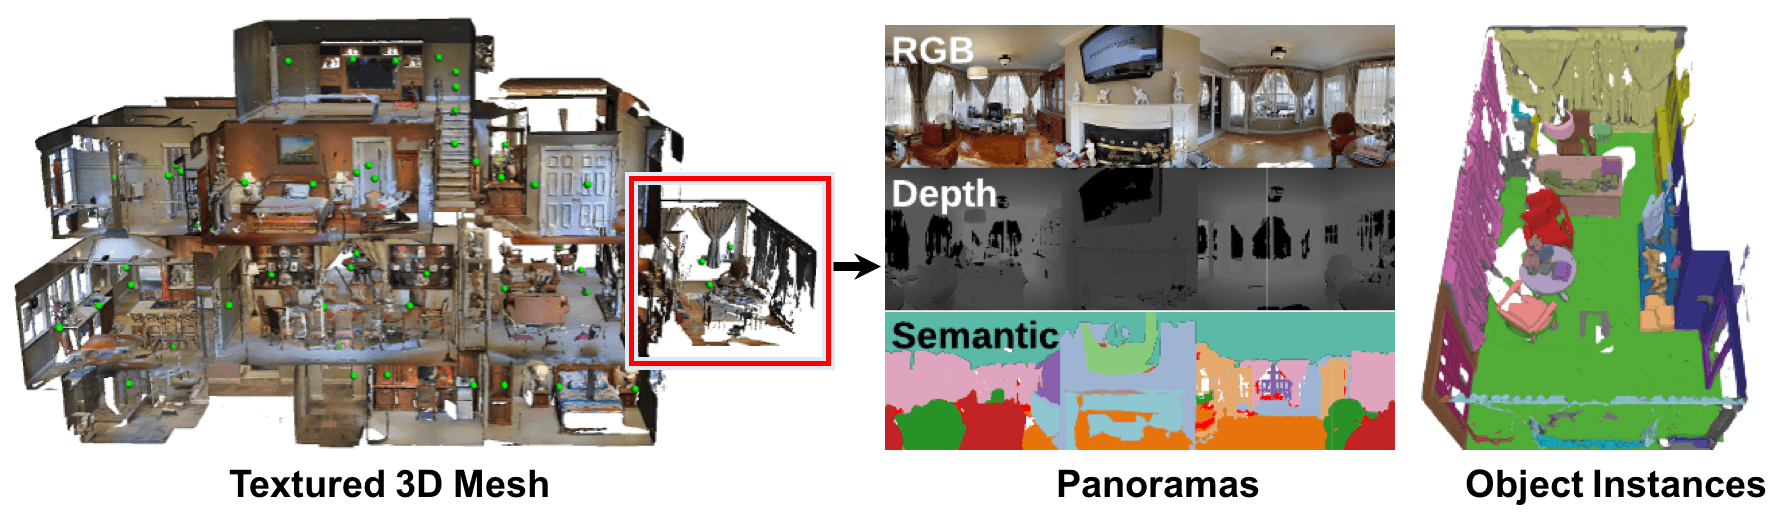
\includegraphics[width=\textwidth]{imagenes/cap4/matterport.png}
    \caption{Modelos 3D de \textit{Matterport3D}, y panorámicas asociadas \cite{Matterport3D}.}
    \label{fig:chap4-matterport}
\end{figure}
	
	\item \textbf{\textit{Gibson} \cite{xiazamirhe2018gibsonenv}:}	\textit{Gibson} es un conjunto de datos originalmente diseñado para el simulador \textit{Gibson}, generado a partir de escaneo 3D y reconstrucción de espacios del interior de edificios. El conjunto de datos cuenta con \textbf{572} edificios, llegando a un total de \textbf{1447} plantas con una superficie total de \textbf{211} kilómetros cuadrados.
	
	Este conjunto de datos incluye información sobre:
	\item Reconstrucciones 3D del escenario, con texturas a partir de las panorámicas.
		\item Panorámicas de color (\textit{RGB}).
		\item Panorámicas de profundidad.
		\item \textit{Normales} de las superficies.
		
	Además, una fracción de los escenarios incluyen anotaciones semánticas sobre los objetos contenidos. Se puede ver un ejemplo de un escenario en la Figura \ref{fig:chap4-gibson}.

\begin{figure}[h]
    \centering
    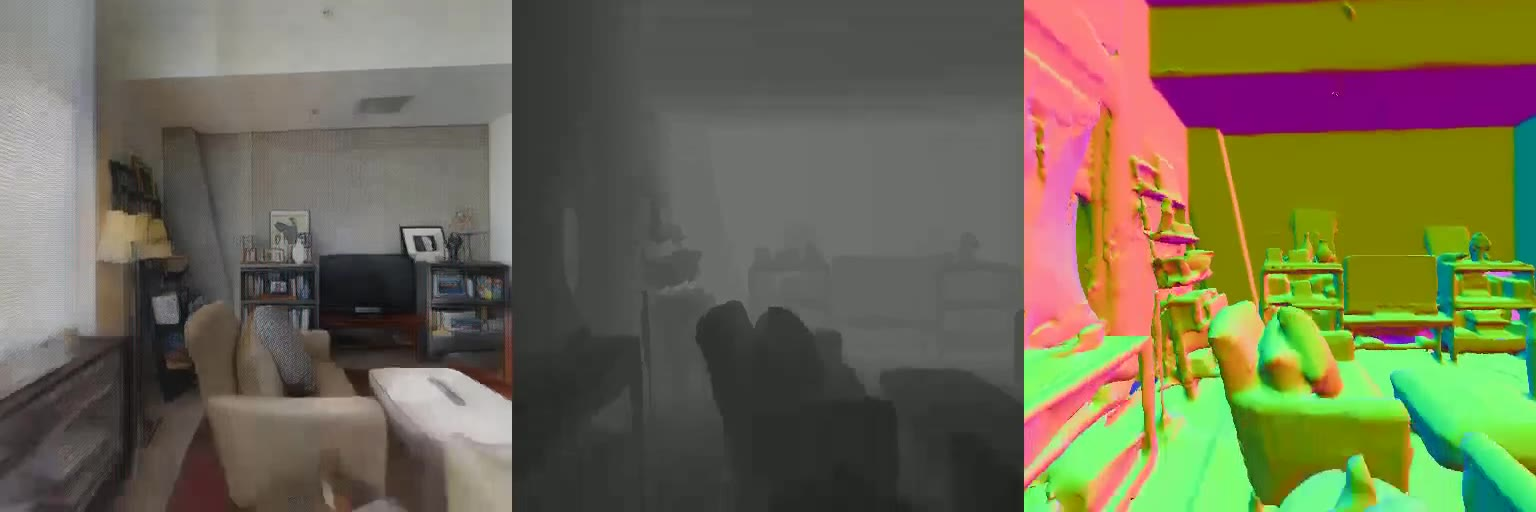
\includegraphics[width=\textwidth]{imagenes/cap4/gibson.jpg}
    \caption{Imagen de color (izquierda), profundidad (centro) y normales (derecha) de un escenario de \textit{Gibson} \cite{xiazamirhe2018gibsonenv}.}
    \label{fig:chap4-gibson}
\end{figure}

\end{itemize}

En general, tanto \textit{Matterport3D} como \textit{Gibson} son conjuntos de datos extensos con información similar, pudiendo cumplir las mismas funciones. Ahora bien, \textit{Gibson} se considera un conjunto más \textit{"fácil"} para el entrenamiento de agentes físicos \cite{habitat19iccv}, al estar formado por escenarios más pequeños.

\textit{Habitat 2.0} añadió soporte a \textbf{dos} conjuntos de datos adicionales por defecto:
\begin{itemize}
	\item \textbf{\textit{ReplicaCAD} \cite{szot2021habitat}:} \textit{ReplicaCAD} es una recreación del conjunto de datos \textit{Replica} \cite{DBLP:journals/corr/abs-1906-05797}, adaptado para el motor de físicas de \textit{Habitat 2.0}. Se puede ver un ejemplo de esta recreación en la Figura \ref{fig:chap4-replicaCAD}.
	
	El conjunto de datos cuenta con \textbf{6} cuartos (teniendo cada cuarto \textbf{5} variaciones y ruido añadido proceduralmente), donde todos los objetos incluyen simulaciones físicas y anotaciones semánticas.
	
	Este conjunto de datos está diseñado expresamente para tareas de reorganización, no estando preparado para otras tareas como navegación.
	
\begin{figure}[h]
    \centering
    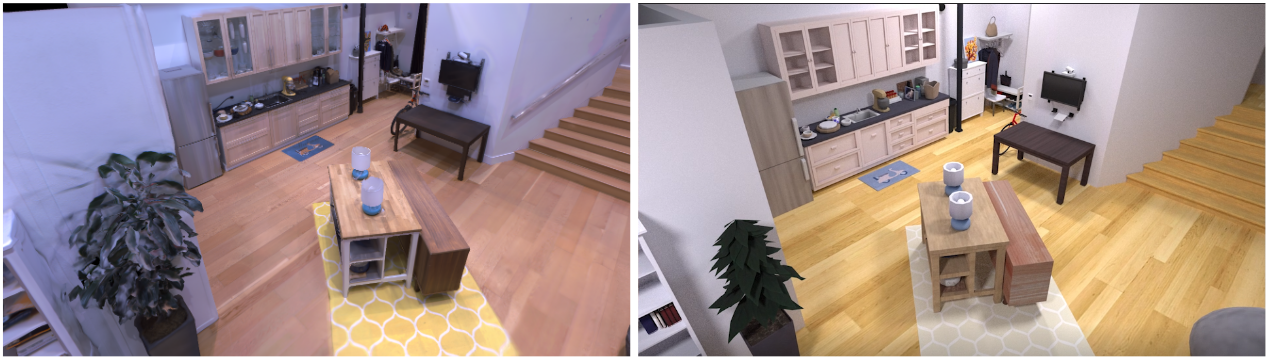
\includegraphics[width=\textwidth]{imagenes/cap4/replicaCAD.png}
    \caption{Escenario original de \textit{Replica} (izquierda) y escenario reconstruido de \textit{ReplicaCAD} (derecha) \cite{szot2021habitat}.}
    \label{fig:chap4-replicaCAD}
\end{figure}	
	
	\item \textbf{\textit{Habitat-Matterport 3D Research Dataset} \cite{habitatmp3d}:} \textit{Habitat-Matterport 3D Research Dataset} (también conocido como \textit{HM3D}) es un conjunto de datos diseñado por el \textit{Facebook AI Research}, generado a partir de imágenes tomadas con cámaras \textit{Matterport}.
	
	Actualmente cuenta con \textbf{1000} escenarios 3D realizados con imágenes de alta resolución de edificios residenciales, comerciales, públicos... Esto lo hace el conjunto de datos más grande actualmente, con alrededor de \textbf{365} kilómetros cuadrados de superficie.
	
	El conjunto de datos ofrece la siguiente información:
	
	\begin{itemize}
		\item Reconstrucciones 3D del escenario, con texturas a partir de las panorámicas.
		\item Panorámicas de color (\textit{RGB}).
		\item Panorámicas de profundidad.
		\item Anotaciones de metadatos de cada escena (incluyendo información como la valoración, el numero de pisos y cuartos, la cantidad de ruido en el escenario...)
	\end{itemize}
	
	Se puede observar un ejemplo de un escenario con la información en la Figura \ref{fig:chap4-hm3d}.	
	
	\begin{figure}[h]
    \centering
    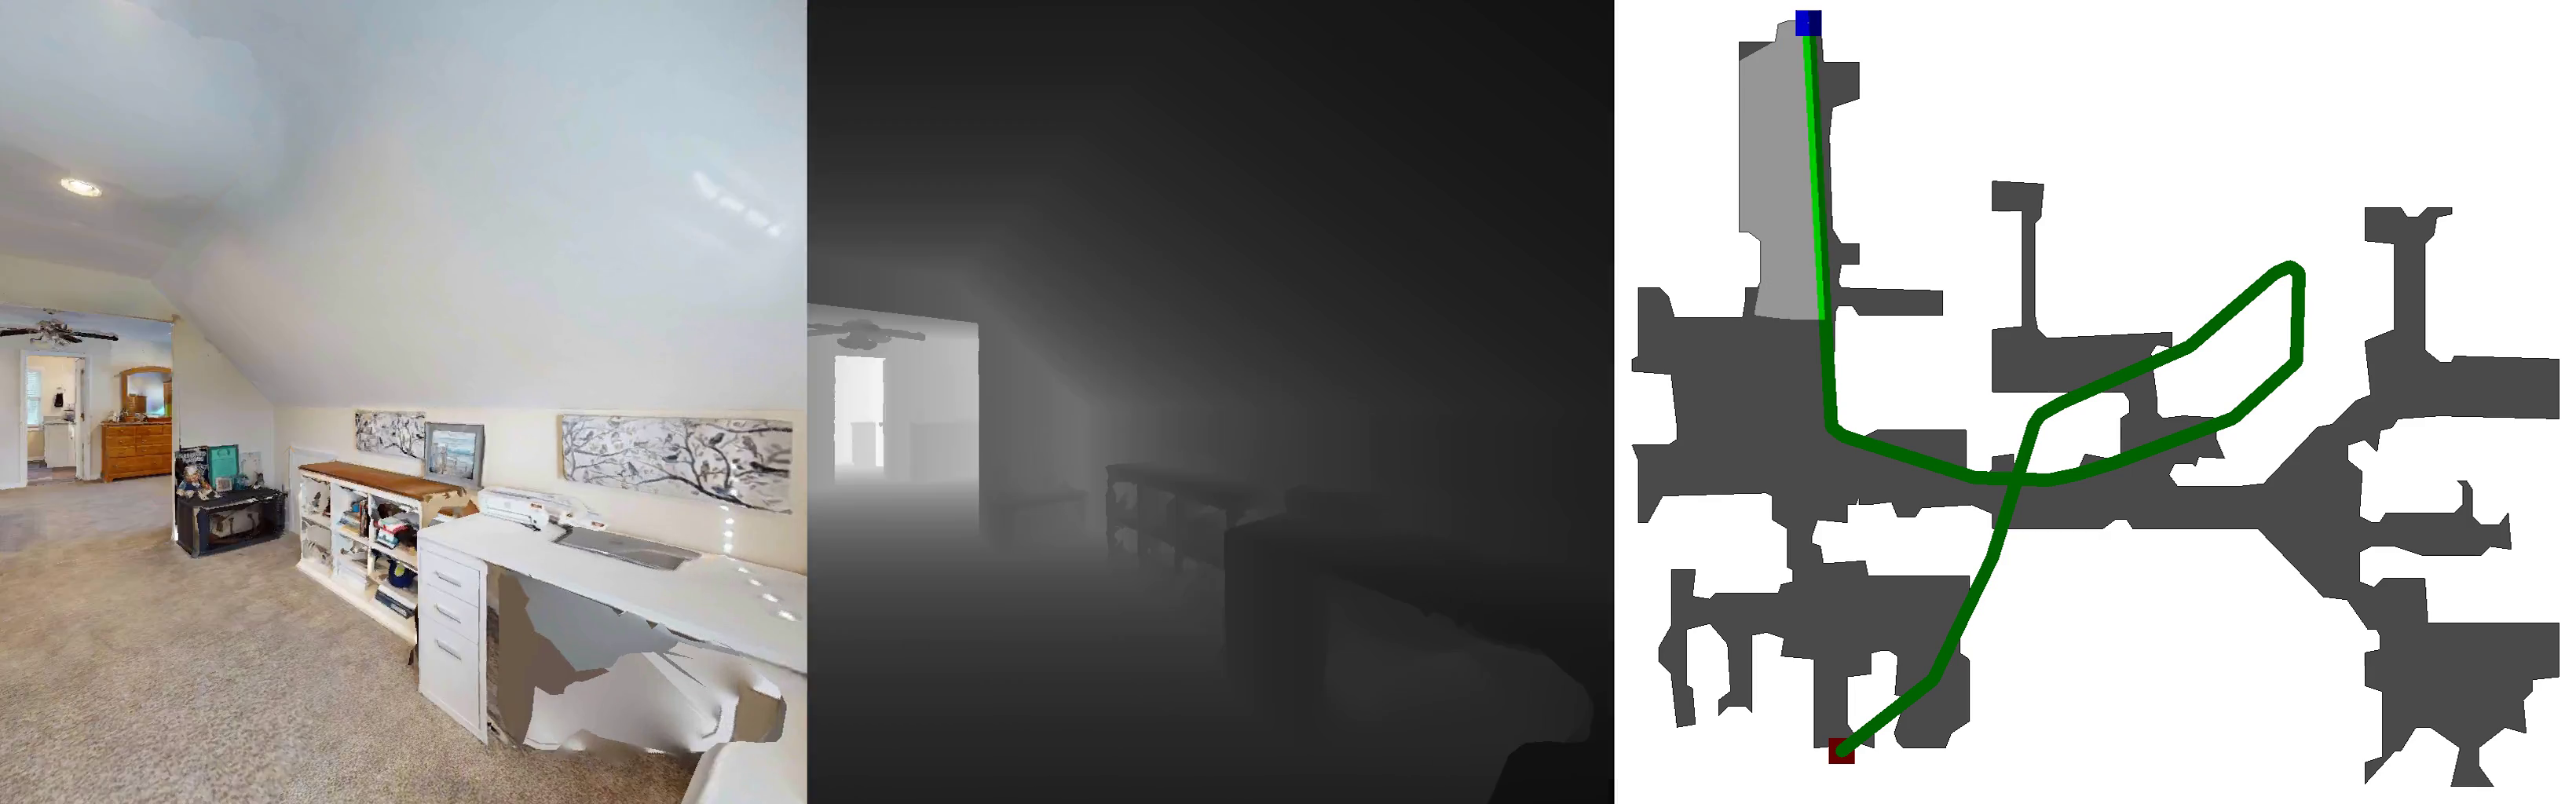
\includegraphics[width=\textwidth]{imagenes/cap4/hm3d.png}
    \caption{Imagen de color (izquierda), profundidad (centro) y mapa (derecha) de una escena de \textit{HM3D} \cite{habitatmp3d}.}
    \label{fig:chap4-hm3d}
\end{figure}	
\end{itemize}

El conjunto \textit{HM3D} ofrece características y dificultad similar a \textit{Matterport3D} y \textit{Gibson}, siendo su principal diferencia la cantidad de escenarios disponibles.

\subsubsection{Estructura de los conjuntos de datos}

Para trabajar con conjuntos de datos, \textit{Habitat} espera que se siga una estructura concreta en el árbol de directorios, como se puede ver en la Figura \ref{fig:tree}.

Especificamente, se espera una carpeta base \textit{data} (o un enlace simbólico a la misma) en el mismo directorio que el fichero ejecutable, que debe tener en su interior a su vez dos carpetas:

\begin{figure}[h]
\centering
\begin{forest}
  for tree={
    font=\ttfamily,
    grow'=0,
    child anchor=west,
    parent anchor=south,
    anchor=west,
    calign=first,
    edge path={
      \noexpand\path [draw, \forestoption{edge}]
      (!u.south west) +(7.5pt,0) |- node[fill,inner sep=1.25pt] {} (.child anchor)\forestoption{edge label};
    },
    before typesetting nodes={
      if n=1
        {insert before={[,phantom]}}
        {}
    },
    fit=band,
    before computing xy={l=15pt},
  }
[data
  [scene{\_}datasets
    [(nombre del dataset 1)]
    [...]
    [(nombre del dataset n)]
  ]
  [datasets
    [(tarea 1)
    	[(nombre del dataset 1)
    		[(version del dataset)
    			[train]
    			[val]
    		]
    	]
    	[...]
    	[(nombre del dataset n)]
    ]
    [...]
    [(tarea n)]
  ]
]
\end{forest}
\caption{Ejemplo de árbol de directorios de la carpeta \textit{data}.}
\label{fig:tree}
\end{figure}

\begin{itemize}
	\item \textbf{\textit{scene{\_}datasets}:} Esta carpeta contiene los modelos 3D de las escenas de cada conjunto de datos, estando cada conjunto contenido en una carpeta con su nombre. Los escenarios en general se encuentran en formato \textit{.glb}, aunque pueden usarse otros.
	\item \textbf{\textit{datasets}:} Esta carpeta contiene, para cada tarea, la definición de todos los escenarios (posición inicial, meta...) para cada conjunto de datos. \textit{Habitat Lab} ofrece estos conjuntos, pudiendo descargarse desde el repositorio de \textit{GitHub}. 
\end{itemize}

\subsection{Acciones}

Una \textbf{acción} \textit{(action)} representa una acción que el agente puede realizar en el entorno mientras resuelve una tarea.

Las acciones derivan de la clase base \textit{SimulatorTaskAction}. Cada tarea incluye un conjunto de acciones posibles, siendo las principales acciones relacionadas con navegación las siguientes:

\begin{itemize}
	\item \textbf{\textit{MOVE{\_}FORWARD}:} Mueve el agente hacia adelante. Por defecto, el agente avanza $0.25m$.
	\item \textbf{\textit{TURN{\_}RIGHT / TURN{\_}LEFT}:} Gira al agente sobre sí mismo hacia la derecha o la izquierda respectivamente. Por defecto, el agente rota $10$ grados.
	\item \textbf{\textit{LOOK{\_}UP / LOOK{\_}DOWN}:} Mueve el ángulo de visión del agente hacia arriba o hacia abajo respectivamente. Por defecto, el ángulo se mueve $15$ grados.
	\item \textbf{\textit{TELEPORT}:} Teletransporta al agente a las coordenadas indicadas.
	\item \textbf{\textit{VELOCITY{\_}CONTROL}:} Ajusta la velocidad lineal y angular del agente a la indicada.
	\item \textbf{\textit{STOP}:} Finaliza el episodio actual, evaluando si ha sido un éxito o no dependiendo de las métricas usadas. Esta acción es importante para evaluar el rendimiento de los agentes en tareas de navegación \cite{DBLP:journals/corr/abs-1807-06757}.
\end{itemize}

Existen otras acciones relacionadas con otras tareas (como \textit{VLN}, \textit{EQA} o \textit{reorganización}) que no han sido mencionadas al no ser relevantes para el problema de navegación a resolver.

\subsection{Sensores}

Un \textbf{sensor} proporciona información del entorno al agente. Esta información es recibida tras cada paso de simulación realizado (siendo el valor devuelto por el método \textit{step} de los entornos).

La clase \textit{Sensor} implementa la funcionalidad básica, existiendo gran cantidad de sensores para diversas tareas. A continuación se describen algunos de los sensores más importantes para navegación:

\begin{itemize}
	\item \textbf{Cámaras:} Las cámaras ofrecen información visual (imágenes) del entorno, devuelta en forma de matriz de valores numéricos. Por defecto, las cámaras apuntan hacia el frente del agente con un ángulo de visión de 90 grados. Existen tres tipos básicos de cámaras disponibles:
	\begin{itemize}
		\item \textbf{Cámara de color (\textit{RGB{\_}SENSOR}):} Devuelve una imagen en color (siguiendo el formato RGB).
		\item \textbf{Cámara de profundidad (\textit{DEPTH{\_}SENSOR}):} Devuelve una imagen en escala de grises representando la profundidad percibida por la cámara. Los valores de esta imagen se representan en forma de números reales en el rango $[0, 1]$ siendo $0.0$ lo más cercano a la cámara y $1.0$ lo más lejano.
		\item \textbf{Cámara semántica (\textit{SEMANTIC{\_}SENSOR}):} Devuelve una imagen seccionada en categorías semánticas (como suelo, techo...). Cada categoría semántica tiene un color asociado. Esta cámara solo puede usarse en conjuntos de datos compatibles con anotaciones semánticas. 
	\end{itemize}
	
	Se puede ver un ejemplo de la misma escena vista desde los tres tipos de cámaras en la Figura \ref{fig:chap4-cameras}.
	
	\begin{figure}[h]
    \centering
    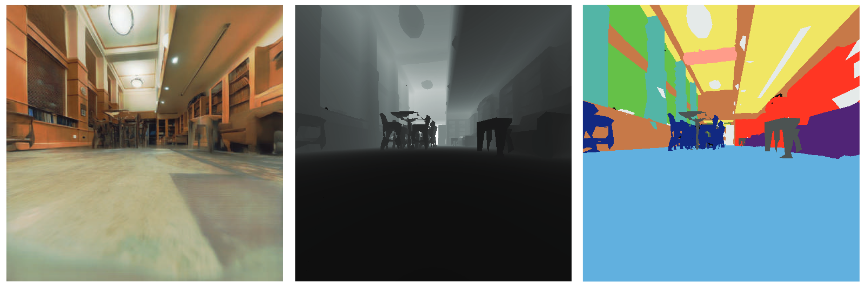
\includegraphics[width=\textwidth]{imagenes/cap4/cameras.png}
    \caption{Imagen de color (izquierda), profundidad (centro) y semántica (derecha) de una escena de \textit{Gibson} \cite{xiazamirhe2018gibsonenv}.}
    \label{fig:chap4-cameras}
\end{figure}		

	\item \textbf{Indicadores de posición:} Los indicadores de posición dan información al agente sobre su propia posición o la de la meta. Estos sensores son exclusivos de tareas de navegación, siendo los principales:
	\begin{itemize}
	\item \textbf{\textit{GPS (GPS{\_}SENSOR)}:} Indica las coordenadas actuales del agente.
	\item \textbf{Brújula \textit{(COMPASS{\_}SENSOR}):} Indica la orientación actual del agente.
	\item \textbf{Meta \textit{(POINTGOAL{\_}SENSOR)}:} Indica las coordenadas de la meta.
	\item \textbf{Combinado \textit{(POINTGOAL{\_}WITH{\_}GPS{\_}COMPASS{\_}SENSOR)}:} Una combinación de los tres sensores anteriores, indicando las coordenadas de agente y meta y el ángulo del agente. Además, indica la distancia del agente a la meta.
	\item \textbf{Proximidad \textit{(PROXIMITY{\_}SENSOR)}:} Indica la distancia en metros del obstáculo más cercano al agente.
	\end{itemize}
\end{itemize}

\subsection{Métricas}

Una \textbf{métrica} \textit{(measure)} indica información sobre la tarea que se está realizando. Esta información no está disponible para el agente, sino que se usa para evaluar el éxito de los episodios y para obtener estadísticas del proceso.

La clase \textit{Measure} implementa la funcionalidad básica de las métricas, de la que se debe derivar cualquier otra métrica definida. Además, las métricas se definen para tareas específicas, no pudiendo usarse métricas de una tarea en otra distinta. Las principales métricas usadas en navegación son:

\begin{itemize}
	\item \textbf{Distancia a la meta \textit{(DISTANCE{\_}TO{\_}GOAL)}:} Indica la distancia actual en metros entre el agente y la meta.
	\item \textbf{Éxito \textit{(SUCCESS)}:} Valor booleano que indica si el agente actualmente ha alcanzado la meta o no. No es posible usar esta métrica sin incluir la distancia a la meta.
	\item \textbf{\textit{Success weighted by Path Length (SPL)}:} Métrica originalmente propuesta por Peter Anderson \textit{et al.} \cite{DBLP:journals/corr/abs-1807-06757} y diseñada para ser usada en un conjunto de episodios, indica un valor en el rango $[0, 1]$ calculado a partir de la tasa de éxito ponderada por la distancia recorrida para alcanzar ésta. Esta métrica se calcula usando la siguiente fórmula:
	\[ \frac{1}{N} \sum^{N}_{i=1} S_{i} \frac{l_i}{max(p_i,l_i)} \]
	
	Donde $N$ es el número total de episodios, $S_i$ es un valor binario ($1$ si el episodio es un éxito, 0 en otro caso), $l_i$ es la distancia más corta entre la posición inicial y la meta en el episodio $i$, y $p_i$ es la distancia recorrida por el agente.
	
	Esta métrica es una mejor estimación del rendimiento de los agentes, al ser capaz de penalizar a los agentes por tomar rutas subóptimas. Ahora bien, es una métrica estricta, siendo un valor de $0.5$ suficiente para esperar un buen rendimiento por parte del agente.
	
	\item \textbf{\textit{SPL} suavizado (\textit{SOFT{\_}SPL}):} Variante de \textit{SPL} diseñada para ser una métrica menos estricta. La diferencia es que el valor $S_i$ pasa de ser binario a lineal. El nuevo valor de la métrica es:
	\[ \frac{1}{N} \sum^{N}_{i=1} S_{i} \frac{l_i}{max(p_i,l_i)} \]
	Donde $N$ es el número total de episodios, $l_i$ es la distancia más corta entre la posición inicial y la meta en el episodio $i$, $p_i$ es la distancia recorrida por el agente y $S_i$ es:
	\[S_i = 1 - \frac{p^{euc}_i}{l^{euc}_i}\]
	Donde $l^{euc}_i$ es la distancia euclidiana entre la posición inicial y la final, y $p^{euc}_i$ es la distancia euclidiana entre el agente y la posición final. Esto es equivalente al porcentaje de la distancia que ha recorrido el agente (donde $S_i = 0$ equivale a un agente que no se ha acercado a la meta y $S_i=1$ equivale a un agente que ha alcanzado la meta).
	
	\item \textbf{Colisiones \textit{(COLLISIONS)}:} Indica el número total de colisiones hasta el momento y si el agente está colisionando actualmente.
	\item \textbf{Mapa del escenario \textit{(TOP{\_}DOWN{\_}MAP)}:} Mapa en plano cenital donde se muestra el escenario entero. Además, se muestra la posición actual del agente, el camino recorrido hasta el momento por el agente (en azul) y la ruta óptima desde la posición inicial hasta la meta (en verde). Se puede ver un ejemplo de un mapa en la Figura \ref{fig:chap4-topdownmap}.
	
\begin{figure}[h]
    \centering
    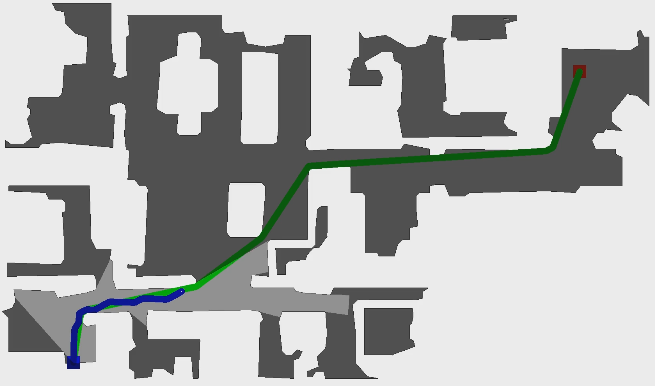
\includegraphics[width=0.6\textwidth]{imagenes/cap4/topdownmap.png}
    \caption{Mapa de un escenario de \textit{HM3D} \cite{habitatmp3d}.}
    \label{fig:chap4-topdownmap}
\end{figure}			
	
\end{itemize}

Las métricas generalmente son devueltas por el método \textit{get{\_}info} de los entornos, y son principalmente usadas durante tareas de aprendizaje por refuerzo.

\subsection{Entrenadores}

Un \textbf{entrenador} \textit{(trainer)} es una clase conteniendo los algoritmos y métodos necesarios para el entrenamiento de un agente con aprendizaje (ya sea aprendizaje por refuerzo o aprendizaje por imitación). A pesar de no estar mencionados directamente en la documentación, los entrenadores son una de las partes más esenciales del uso del simulador, al ser la principal forma de realizar el proceso de entrenamiento.

Si bien \textit{Habitat Lab} no ofrece por defecto ningún entrenador, \textit{Habitat Baselines} incluye la clase \textit{BaseTrainer} (con los métodos básicos que deben heredar los entrenadores) y \textit{BaseRLTrainer} (una subclase con métodos usados por problemas de aprendizaje por refuerzo).

Los entrenadores de aprendizaje por refuerzo deben heredar de la clase \textit{BaseRLTrainer} y ser desarrollados específicamente para el algoritmo usado, teniendo que implementar los siguientes métodos:

\begin{itemize}
	\item \textbf{\textit{save{\_}checkpoint(nombre) / load{\_}checkpoint(ruta)}:} Guardan un \textit{checkpoint} con el nombre especificado o cargan un \textit{checkpoint} con la ruta especificada, respectivamente.
	
	Para \textit{Habitat}, se suele entender un \textit{checkpoint} como un fichero comprimido conteniendo los \textbf{pesos de la red neuronal} usada durante el entrenamiento y una copia del \textbf{fichero de configuración} usado. De esta forma, es posible reanudar el entrenamiento en cualquier momento garantizando que no hay modificaciones en el entorno.
	
	\item \textbf{\textit{{\_}eval{\_}checkpoint(ruta)}:} Evalúa el rendimiento de un \textit{checkpoint} (indicado por la ruta) en el entorno. Este método es llamado desde un método superior ya implementado, \textit{eval}, que evalúa todos los \textit{checkpoints} realizados. El método se usa principalmente para elegir el \textit{checkpoint} de mayor rendimiento en el conjunto de evaluación.
	
	La forma más típica de evaluar un \textit{checkpoint} es simular uno o varios episodios enteros usando la información contenida en el \textit{checkpoint}, y posteriormente valorar las métricas del entorno para realizar una comparativa. 

	\item \textbf{\textit{train()}:} El método más importante del entrenador, \textit{train} se encarga de:
	\begin{itemize}
		\item Inicializar los modelos y estructuras de datos usadas.
		\item Simular los episodios del agente.
		\item Aplicar el algoritmo de aprendizaje, actualizando los modelos conforme son entrenados.
	\end{itemize}
	
	El entrenamiento se realiza en bucle hasta que se cumpla una de las dos condiciones de parada posibles: se alcanza el \textbf{número máximo de pasos} durante todos los episodios, o se realiza el \textbf{número de episodios} indicado. Solo se puede indicar una de las dos condiciones de parada a la vez.
	
	Por lo general, el método de entrenamiento sigue el pseudocódigo de la Figura \ref{alg:train}. Este bucle se puede modificar para añadir otras acciones que sea necesario realizar (como actualizaciones durante el episodio o registro de información).
	
	\begin{figure}[h]
\begin{algorithm}[H]
\SetAlgorithmName{Algoritmo}{algoritmo}{Lista de algoritmos}
\caption{Bucle principal de entrenamiento}
\textbf{1.} Inicializa las estructuras de datos necesarias para el entrenamiento, los contadores globales de pasos $num\_steps\_done$ y actualizaciones $num\_updates\_done$, y los modelos a entrenar.\\
\textbf{2.} Mientras no se cumpla la condición de parada (número máximo de pasos o número de actualizaciones):\\
\Indp \textbf{2.1.} Prepara el escenario (a través del método \textit{reset} del entorno)\\
\textbf{2.2.} Mientras no haya finalizado el episodio:\\
\Indp \textbf{2.2.1.} El agente percibe el estado del escenario a través de los sensores.\\
\textbf{2.2.2.} El agente procesa el estado, actualizando su modelo si es necesario, y eligiendo una acción.\\
\textbf{2.2.3.} El agente aplica la acción (a través del método \textit{step} del entorno).\\
\textbf{2.2.4.} Incrementa el contador global de pasos $num\_steps\_done$.\\
\Indm \textbf{2.3.} Actualiza el modelo.\\
\textbf{2.4.} Si es necesario, guarda un \textit{checkpoint} del estado actual del modelo.\\
\textbf{2.5.} Incrementa el contador global de actualizaciones $num\_updates\_done$.
\end{algorithm}
\hrule
\caption{Pseudocódigo del bucle principal de entrenamiento.}
\label{alg:train}
\end{figure}
\end{itemize}


\textit{BaseRLTrainer} además incluye varios métodos ya implementados para facilitar el desarrollo del entrenamiento y la comprobación de las condiciones:

\begin{itemize}
	\item \textbf{\textit{is{\_}done()}:} Devuelve un valor booleano \textbf{verdadero} si se ha cumplido la condición de parada (ya sea número de pasos o de episodios), o \textbf{falso} en otro caso. Este método se usa para controlar el bucle general de entrenamiento.
	\item \textbf{\textit{should{\_}checkpoint()}:} Devuelve un valor booleano \textbf{verdadero} si es necesario realizar un \textit{checkpoint}, o \textbf{falso} en otro caso.
	
	Este método calcula automáticamente el porcentaje de entrenamiento realizado, y si es necesario realizar un \textit{checkpoint} en base a dicho porcentaje (a partir del número de \textit{checkpoints} que se ha especificado en el fichero de configuración).
\end{itemize}

En el trabajo se ha implementado un entrenador personalizado (\textit{ReactiveNavigationTrainer}) como subclase de \textit{BaseRLTrainer}, implementando un algoritmo de aprendizaje por refuerzo via \textit{Deep Q-Learning}.

\subsection{Agentes}

Un \textbf{agente} (\textit{agente}) es un contenedor para los modelos entrenados, diseñado para ser usado con los \textit{benchmarks} de \textit{Habitat}.

Los agentes deben heredar de la clase \textit{Agent}, e implementar los dos siguientes métodos:

\begin{itemize}
	\item \textbf{\textit{reset()}:} Prepara al agente para el inicio de un nuevo episodio.
	\item \textbf{\textit{act(observaciones)}:} A partir de las observaciones, el agente debe devolver una acción a realizar en forma de diccionario $\{action="accion\_elegida"\}$.
\end{itemize}

Estos métodos son llamados automáticamente por el entorno contenido en el \textit{benchmark}.

\textit{Habitat Baselines} ofrece algunos agentes preconstruidos (principalmente agentes heurísticos para funcionar como \textit{benchmark} y un agente de aprendizaje aplicando \textit{PPO}). En este trabajo se ha diseñado un agente propio (\textit{ReactiveNavigationAgent}) para evaluar el rendimiento de la propuesta.

En contra de lo que pueda dar a entender el nombre del concepto, los agentes no tienen ninguna relación con los agentes físicos simulados, y su uso se limita exclusivamente a \textit{benchmarks}.

\subsection{\textit{Benchmarks}}

\textit{Habitat} ofrece por defecto un \textit{benchmark} con el que se puede evaluar el rendimiento de los agentes ya entrenados. El benchmark recibe como entrada un agente (definido previamente) y el número de episodios que se quiere evaluar (por defecto todos los posibles), y se encarga de:

\begin{itemize}
	\item Crear y gestionar el entorno (usando un entorno \textit{Env}).
	\item Simular internamente los episodios, usando los métodos del entorno y del agente.
	\item Obtener las métricas de cada episodio realizado.
\end{itemize}

El \textit{benchmark} devuelve como resultado final el valor medio de cada métrica tras todos los episodios evaluados, para poder ser analizado y comparado con otros agentes.

\subsection{Ficheros de configuración}

\textit{Habitat} usa un \textbf{fichero de configuración} para cargar todos los parámetros necesarios para su funcionamiento. Este fichero es, junto a los entrenadores, una de las partes más importantes del uso del simulador, pese a no estar recogida en la documentación.

Los ficheros de configuración son documentos en formato \textit{YAML} \cite{yaml} divididos en bloques. Dentro de cada bloque hay pares de clave - valor que se corresponden al parámetro a configurar (clave) y el valor asignado a ese parámetro (valor).

Los principales bloques del fichero de configuración son:

\begin{itemize}
	\item \textbf{ENVIRONMENT:} En este bloque se incluyen parámetros relativos al entorno, incluyendo la forma en la que se ordenan los episodios o las duraciones máximas de éstos. Algunas de las claves principales de éste bloque son:
	
	\begin{itemize}
		\item \textbf{MAX{\_}EPISODE{\_}STEPS:} Pasos máximos que puede dar un agente en un episodio. Si se supera este valor, el episodio se finaliza inmediatamente.
		\item \textbf{MAX{\_}EPISODE{\_}SECONDS:} Duración máxima del episodio en segundos. Si se supera este valor, el episodio se finaliza inmediatamente.
	\end{itemize}
	
	\item \textbf{SIMULATOR:} En este bloque se incluyen parámetros relativos al simulador y al agente, como los sensores a usar o los parámetros de éstos. Algunas de las claves principales de este bloque son:
	
	\begin{itemize}
		\item \textbf{AGENT{\_}0:} Sub-bloque donde se encuentra la información sobre el agente. Su clave más importante es \textbf{SENSORS}, donde se indica en una lista (entre corchetes) los sensores a usar.
		\item \textbf{RGB{\_}SENSOR / DEPTH{\_}SENSOR:} Sub-bloques donde se especifican los parámetros de los sensores, \textbf{WIDTH} (anchura en píxeles de la imagen devuelta por el sensor) y \textbf{HEIGHT} (altura en píxeles). El resto de sensores se pueden configurar de una forma similar.
	\end{itemize}
	
	\item \textbf{DATASET:} Contiene información sobre el conjunto de datos a utilizar. Algunas de las claves principales de este bloque son:
	\begin{itemize}
		\item \textbf{TYPE:} Tipo de conjunto de datos a utilizar. Este tipo se debe corresponder con el tipo de tarea a realizar.
		\item \textbf{DATA{\_}PATH:} Ruta a los ficheros del conjunto de datos a utilizar. Se puede usar la palabra $\{split\}$ para indicar una sección de la ruta que se sustituye por el valor de la variable \textbf{SPLIT}.
		\item \textbf{SPLIT:} Partición del conjunto de datos a utilizar. Por defecto, las particiones son \textbf{train} (entrenamiento) y \textbf{val} (validación).
	\end{itemize}
	
	\item \textbf{TASK:} Contiene información sobre la tarea a realizar y las métricas a utilizar. Algunas de las claves principales de este bloque son:
	\begin{itemize}
		\item \textbf{SENSORS:} Lista de métricas a usar para la valoración de la tarea. Estas métricas pueden personalizarse en sub-bloques, de forma similar a la configuración de los sensores.
		\item \textbf{SUCCESS{\_}DISTANCE:} Distancia (en metros) a la que tiene que estar el agente de la meta para que se considere que el episodio se ha completado con éxito.
	\end{itemize}
	
	\item \textbf{RL:} Contiene información relacionada con el aprendizaje por refuerzo, para ser usada por los entrenadores. Esta sección es opcional y no tiene una estructura fija, pudiendo añadir las claves deseadas para ser leídas posteriormente.
	
	\item \textbf{Claves sin bloque:} Se pueden indicar claves fuera del resto de bloques, quedando a la altura de la raíz. Estas claves en general están relacionadas con configuraciones para los procesos de entrenamiento y registro de datos, siendo algunas de las principales:
	\begin{itemize}
		\item \textbf{BASE{\_}TASK{\_}CONFIG{\_}PATH:} Ruta al fichero de configuración base. Si se especifica este valor, los valores contenidos en este fichero se fusionarán con los del fichero indicado. Permite crear una configuración base sobre la que crear variaciones.
		\item \textbf{TRAINER{\_}NAME / ENV{\_}NAME:} Identificador del entrenador o del entorno a utilizar, respectivamente. Estos identificadores se usan para obtener la clase adecuada del registro (como se verá después).
		\item \textbf{TOTAL{\_}NUM{\_}STEPS / NUM{\_}UPDATES:} Número máximo de pasos o actualizaciones a realizar durante el entrenamiento. El entrenamiento dura hasta que se alcanza uno de estos valores. Solo puede aparecer una de las dos claves en el fichero.
		\item \textbf{NUM{\_}CHECKPOINTS:} Número total de \textit{checkpoints} a realizar durante el proceso de entrenamiento.
		\item \textbf{CHECKPOINT{\_}FOLDER:} Carpeta en la que se almacenarán los \textit{checkpoints} realizados.
	\end{itemize}
	
	Existen más claves dentro de esta categoría, pudiendo observarse en los ficheros de configuración de ejemplo.
\end{itemize}

Se puede ver un ejemplo de un fichero de configuración para una tarea de navegación usando \textit{Gibson} en la Figura \ref{fig:chap4-conf}. Además, se pueden ver los ficheros de configuración desarrollados (documentados en inglés) en el Anexo B (Ficheros de configuración).

\begin{figure}[!ht]
\centering
\begin{lstlisting}[language=yaml]
ENVIRONMENT:
  MAX_EPISODE_STEPS: 500
SIMULATOR:
  AGENT_0:
    SENSORS: ['RGB_SENSOR']
  HABITAT_SIM_V0:
    GPU_DEVICE_ID: 0
  RGB_SENSOR:
    WIDTH: 256
    HEIGHT: 256
  DEPTH_SENSOR:
    WIDTH: 256
    HEIGHT: 256
TASK:
  TYPE: Nav-v0
  SUCCESS_DISTANCE: 0.2

  SENSORS: ['POINTGOAL_WITH_GPS_COMPASS_SENSOR']
  POINTGOAL_WITH_GPS_COMPASS_SENSOR:
    GOAL_FORMAT: "POLAR"
    DIMENSIONALITY: 2
  GOAL_SENSOR_UUID: pointgoal_with_gps_compass

  MEASUREMENTS: ['DISTANCE_TO_GOAL', 'SUCCESS', 'SPL']
  SUCCESS:
    SUCCESS_DISTANCE: 0.2

DATASET:
  TYPE: PointNav-v1
  SPLIT: train
  DATA_PATH: data/datasets/pointnav/gibson/v1/{split}/{split}.json.gz
\end{lstlisting}
\caption{Fichero de configuración por defecto para tareas de navegación usando \textit{Gibson}.}
\label{fig:chap4-conf}
\end{figure}

El simulador no trabaja directamente con el fichero de configuración, sino que primero convierte el contenido del fichero a un objeto de la clase \textit{Config}. Este objeto contiene todos los valores del fichero en forma de diccionario, y se puede obtener de la siguiente forma:

\begin{itemize}
	\item \textbf{Método \textit{get{\_}config(ruta)} de \textit{Habitat Lab}:} Este método (disponible en el fichero \textit{habitat/config/default.py}) genera una instancia de \textit{Config} a partir de una serie de valores por defecto y los valores indicados en el fichero de configuración. Es recomendable usar este método para configuraciones relacionadas con \textit{benchmarks}.
	\item \textbf{Método \textit{get{\_}config(ruta)} de \textit{Habitat Baselines}:} Este método se diferencia del anterior en tres puntos:
	\begin{itemize}
		\item Incluye valores por defecto de aprendizaje por refuerzo.
		\item Es capaz de cargar los valores de otro fichero de configuración (indicado con la clave \textit{BASE{\_}TASK{\_}CONFIG{\_}PATH}.
		\item Almacena los valores de los cuatro bloques principales (\textit{ENVIRONMENT, SIMULATOR, DATASET} y \textit{TASK}) bajo un nuevo bloque llamado \textit{TASK{\_}CONFIG}.
	\end{itemize}	 
	Es recomendable usar este método para configuraciones de entrenadores.
\end{itemize}

\subsection{Registros}

Un \textbf{registro} (\textit{registry}) es un contenedor global y central de información, en el que se almacenan pares de clave y clase asociada a la clave. Estos registros sirven para poder instanciar las clases apropiadas (de simulador, tarea, entorno...) a partir de sus identificadores, siendo especialmente útil para cargar las clases indicadas en el fichero de configuración.

Los registros funcionan usando \textbf{decoradores}, funciones que se llaman durante la definición de las clases y que las registran para poder acceder a ellas posteriormente desde cualquier punto del código.

Por defecto, \textit{Habitat} incluye dos registros, cada uno almacenando información distinta:

\begin{itemize}
	\item \textbf{Registro \textit{Registry} de \textit{Habitat Lab}:} El registro principal en el que se incluye información sobre:
	\begin{itemize}
		\item \textbf{Tareas}, usando el decorador \textit{@registry.register{\_}task}.
		\item \textbf{Acciones}, usando el decorador \textit{@registry.register{\_}task{\_}action}.
		\item \textbf{Simuladores}, usando el decorador \textit{@registry.register{\_}simulator}.
		\item \textbf{Sensores}, usando el decorador \textit{@registry.register{\_}sensor}.
		\item \textbf{Métricas}, usando el decorador \textit{@registry.register{\_}measure}.
		\item \textbf{Conjuntos de datos}, usando el decorador \textit{@registry.register{\_}dataset}.
	\end{itemize}
	\item \textbf{Registro \textit{BaselineRegistry} de \textit{Habitat Baselines}:} Un registro adicional pensado para almacenar las clases creadas por el usuario, incluye información sobre:
	\begin{itemize}
		\item \textbf{Entornos}, usando el decorador \textit{@baseline{\_}registry.register{\_}env}.
				\item \textbf{Entrenadores}, usando el decorador \textit{@baseline{\_}registry.register{\_}trainer}.
				\item \textbf{Políticas de acciones}, usando el decorador \textit{@baseline{\_}registry.register{\_}policy}.
	\end{itemize}
\end{itemize}

\section{Instalación de \textit{Habitat}}

El proceso de instalación de \textit{Habitat} puede resultar complicado debido a la gran cantidad de componentes y versiones específicas necesarias. Por eso, en esta sección se indican los pasos necesarios para instalar el entorno de \textit{Habitat}, remarcando los requisitos de versiones necesarios para el funcionamiento adecuado.

\subsection{Requisitos}

El entorno de \textit{Habitat} requiere versiones específicas de 

\begin{itemize}
	\item \textbf{Python:} Versión superior a \textit{3.6.0} (recomendable usar \textit{3.6.10}).
	\item \textbf{cmake:} Versión superior a \textit{3.10} (recomendable usar \textit{3.14.0}).
	\item \textbf{Sistema operativo:} Si bien \textit{Habitat Sim} incluye soporte para Windows, es recomendable usar alguna distribución de \textit{Linux} con soporte para \textit{CUDA}. En este trabajo se ha utilizado \textbf{Ubuntu 20.04}.
	\item \textbf{Tarjeta gráfica:} En caso de ser necesaria, se necesita una tarjeta gráfica de \textit{nVidia} que ofrezca soporte para \textit{CUDA}.
	\item \textbf{CUDA:} Se ha usado la versión \textit{11.0} en el trabajo realizado, aunque es posible que dependiendo de la configuración se necesite otra.
\end{itemize}

Además, la instalación de \textit{Habitat Lab} y \textit{Habitat Baselines} instala versiones concretas de diversas librerías de \textit{Python}, por lo que es recomendable instalar \textit{Habitat} en un entorno propio de \textit{Conda} para evitar problemas de compatibilidad. 

\subsection{Proceso de instalación}

Si bien es posible utilizar \textit{dockers} para instalar el entorno del simulador, es recomendable realizar la instalación directamente para garantizar acceso a las actualizaciones. El proceso de instalación en distribuciones de \textit{Linux} se puede dividir en tres pasos principales:

\begin{enumerate}
	\item \textbf{Instalación de CUDA:} Para el uso de \textit{Habitat} y para el entrenamiento adecuado de redes neuronales, es necesaria una instalación correcta y completa de CUDA. Para esto, es necesario:
	\begin{enumerate}
		\item Tener \textit{drivers} \textbf{oficiales} de \textit{nVidia}, actualizados a la versión más moderna. No es necesaria una versión concreta del \textit{driver}.
		\item Instalar \textbf{CUDA}. La guía oficial de instalación en \textit{Linux}\footnote{\url{https://docs.nvidia.com/cuda/cuda-installation-guide-linux/index.html}} incluye los pasos a seguir, mientras que la página de descarga\footnote{\url{https://developer.nvidia.com/cuda-downloads}} ofrece las instrucciones para descargar e instalar CUDA.
		
		Es recomendable seguir los pasos de pre-instalación y post-instalación indicados en la guía oficial, pero seguir los pasos de la página de descarga para la instalación.
		
		\item Instalar \textbf{cuDNN}. La guia oficial de instalación en \textit{Linux}\footnote{\url{https://docs.nvidia.com/deeplearning/cudnn/install-guide/index.html}} incluye los pasos necesarios para instalar cuDNN. Es importante comprobar que las versiones de CUDA y cuDNN instaladas sean compatibles entre sí.
		
		Es necesaria una cuenta de desarrollador de \textit{nVidia} para la descarga de cuDNN.
	\end{enumerate}
	\item \textbf{Instalación de \textit{Habitat Sim}:} La instalación de \textit{Habitat Sim} se hace a través del repositorio de paquetes \textit{Conda}. Además, como se ha comentado previamente, es recomendable crear un entorno propio de \textit{Conda} para evitar problemas de compatibilidades. 
	
	Contando con una instalación válida de \textit{Conda}, los siguientes comandos en una terminal crean un entorno con las versiones adecuadas de \textit{Python} y \textit{cMake} e instalan \textit{Habitat Sim}:

\begin{lstlisting}[language=bash]
# Crea el entorno de Conda con las versiones adecuadas de Python y cMake
conda create -n habitat python=3.6 cmake=3.14.0
# Inicializa el entorno creado
conda activate habitat
# Instala el simulador con soporte para fisicas (withbullet)
conda install habitat-sim withbullet -c conda-forge -c aihabitat
\end{lstlisting}	
	
	\item \textbf{Instalación de \textit{Habitat Lab} y \textit{Habitat Baselines}:} Ya con el simulador instalado, el último paso es instalar la librería \textit{Habitat Lab}. Si bien \textit{Habitat Baselines} es opcional, es muy recomendable su instalación por las utilidades adicionales que ofrece. Los siguientes comandos en una terminal instalan \textit{Habitat Lab} y \textit{Habitat Baselines}:
	
\begin{lstlisting}[language=bash]
# Descarga la version mas reciente del repositorio de Habitat Lab
# El repositorio se descarga en la carpeta actual
git clone --branch stable https://github.com/facebookresearch/habitat-lab.git
# Accede al repositorio descargado
cd habitat-lab
# Instala todos los paquetes de Python necesarios
# Es recomendable realizar la instalacion en el mismo entorno que Habitat Sim
# para evitar incompatibilidades
pip install -r requirements.txt
# Instala Habitat Lab y Habitat Baselines
python setup.py develop --all
\end{lstlisting}	
\end{enumerate}

Para comprobar que la instalación se ha realizado correctamente, \textit{Habitat Lab} ofrece el fichero \textit{examples/example.py}. Si no ha habido ningún problema en la instalación, al ejecutar el fichero se realizará una simulación con un agente de ejemplo ofrecido por defecto por \textit{Habitat}, imprimiendo en la terminal el número de pasos realizado.


\chapter{Diseño del agente}

En este capítulo se detallará el diseño del agente propuesto para la resolución del problema. 

Se empezará presentando la formalización del conocimiento usada (estado, acción y recompensa) y las características físicas del agente. Tras esto, se describirán las dos arquitecturas propuestas para el agente: una primera basada en una red neuronal convolucional, y una segunda basada en una red profunda híbrida. Finalmente, se explicará el proceso de actuación y entrenamiento del agente.

\section{Caracterización del conocimiento}

En esta sección se describe la caracterización del conocimiento realizada, centrándose en los puntos principales del aprendizaje por refuerzo: el \textbf{estado}, las \textbf{acciones} disponibles y las \textbf{recompensas} que recibe el agente. Además, se describen las características del agente propuesto dentro del entorno \textit{Habitat}.

\subsection{Características del agente físico en \textit{Habitat}}

Las características del agente físico simulado son las siguientes:
\begin{itemize}
	\item \textbf{Forma física del agente:} La forma del agente es un \textbf{cilindro} de $1.5$ metros de altura y $0.1$ metros de radio.
	
	Esta forma física no se corresponde a ningún robot real, siendo la del agente por defecto simulado por \textit{Habitat}.
	\item \textbf{Capacidad de movimiento:} El agente únicamente es capaz de desplazarse hacia delante, pudiendo moverse $0.25$ metros en cada paso simulado.
	
	Para cambiar la dirección de su movimiento, el agente necesita rotar sobre si mismo. Ésto lo hace en intervalos de $10$ grados en cada paso simulado. El agente no puede girar y desplazarse en el mismo paso.
	\item \textbf{Sensores disponibles:} El agente cuenta con acceso a los siguientes sensores:
	\begin{itemize}
		\item \textbf{Cámara de profundidad:} Una cámara de profundidad (\textit{DEPTH{\_}SENSOR)} situada a una altura de $1.25$ metros respecto al suelo, apuntando a la dirección en la que se desplaza el agente.
		
		Esta cámara genera imágenes de profundidad de $(256x256)$ píxeles con valores en el rango $[0.0, 1.0]$. La cámara tiene un ángulo de visión de $90$ grados, y es capaz de detectar objetos hasta una distancia de $10$ metros.
		\item \textbf{Brújula y GPS (\textit{POINTGOAL{\_}WITH{\_}GPS{\_}COMPASS{\_}SENSOR}):} Una brújula y un GPS que conocen la posición exacta de la meta en todo momento. Estos sensores ofrecen el \textbf{ángulo} y la \textbf{distancia euclidiana} hasta la meta en forma de valor decimal.
	\end{itemize}
	\item \textbf{Métricas usadas:} El agente ofrece las siguientes métricas para su evaluación posterior:
	\begin{itemize}
		\item \textbf{Distancia hasta la meta}: Un valor numérico que indica la distancia euclidiana hasta la meta (la distancia euclidiana entre el agente y la meta) en metros.
		\item \textbf{Éxito:} Un valor booleano que indica si el agente está en la meta (verdadero) o falso. El agente se considera en la meta si se encuentra a menos de $0.3$ metros de esta.
		\item \textbf{\textit{SPL} y \textit{Soft SPL}:} Dos valores numéricos que indican la métrica de \textit{Success weighted by Path Length} \cite{DBLP:journals/corr/abs-1807-06757} y su variante suavizada. Ambas fórmulas fueron definidas en el Capítulo 4.
	\end{itemize}
\end{itemize}

\subsection{Estado}

El \textbf{estado} (la percepción que tiene el agente del entorno) consta de tres elementos:

\begin{itemize}
	\item \textbf{Imagen de profundidad:} Una imagen en escala de grises representando las observaciones de la cámara de profundidad. Esta imagen tiene un tamaño de $(256 x 256)$ píxeles, con los valores de cada celda en el rango $[0.0, 1.0]$ (donde $0.0$ o negro significa cercanía a la cámara y $1.0$ o blanco significa lejanía). Se puede ver un ejemplo de la imagen en la Figura \ref{fig:chap5-estado}.
	
\begin{figure}[h]
    \centering
    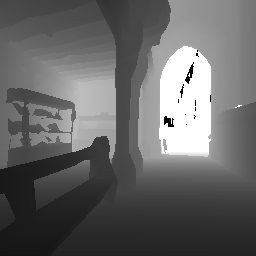
\includegraphics{imagenes/cap5/normalized.png}
    \caption{Ejemplo de imagen de profundidad usada como parte del estado.}
    \label{fig:chap5-estado}
\end{figure}			
			
	Se ha optado por añadir este valor debido al planteamiento del problema. Al buscar diseñar un agente reactivo frente a obstáculos, es importante que el agente sea capaz de percibir cualquier objeto que se encuentre en su camino. Una cámara de profundidad nos permite estimar las distancias a estos obstáculos de forma rápida y simple.	
	

	\item \textbf{Distancia a la meta:} Un valor decimal que representa la distancia actual entre el agente y la meta en metros.
	
	Este valor forma parte del estado al ser parte del cálculo de la recompensa (como se verá posteriormente). Además, es importante que el agente sea capaz de estimar la distancia hasta la meta para que tenga la posibilidad de aprender cuando detenerse.
	
	\item \textbf{Ángulo respecto a la meta:} Un valor decimal que representa el ángulo que debería girar el agente para enfocarse hacia la meta, en radianes. Un valor positivo significa que el agente debería girar hacia la derecha, mientras que un valor negativo significa que el agente debería girar hacia la izquierda.
	
	Si bien este valor no forma parte del cómputo de la recompensa, se ha optado por añadir el ángulo al estado para permitir al agente tener la posibilidad de aprender información respecto a su orientación que no podría aprender en otro caso.
\end{itemize}

Si bien se consideró añadir una \textbf{imagen en color} al estado, finalmente se ha optado por no incluirla. Esto se debe a que la información que añade resulta superflua, ya que la cámara de profundidad incluye toda la información necesaria para el cálculo de obstáculos. Además, los escenarios de interior son complejos con altos niveles de ruido, por lo que una cámara de color podría llevar a sobreajustes (al aprender el aspecto de los interiores frente a los obstáculos).

Un estado se considera \textbf{final} cuando el agente lo finaliza (ya sea por realizar la acción específica de terminar o por superar el número máximo de acciones permitidas). Este estado final puede ser \textbf{exitoso} si la distancia a la meta es menor a un umbral (por defecto $0.3$ metros), o \textbf{fallido} en otro caso.

\subsection{Acciones}

El agente es capaz de realizar \textbf{cuatro} acciones en total:

\begin{itemize}
	\item \textbf{Desplazarse} hacia delante. Por defecto, el desplazamiento es de $0.25$ metros.
	\item \textbf{Girar} hacia la derecha o la izquierda. Por defecto, el giro es de $10$ grados.
	\item \textbf{Finalizar el episodio}. La inclusión de una acción para finalizar el episodio es una de las principales sugerencias de Peter Anderson \textit{et al.} \cite{DBLP:journals/corr/abs-1807-06757} para la evaluación de agentes físicos.
\end{itemize}

Como se comentó en el Capítulo 2 y se puede observar, el agente no es capaz de un movimiento omnidireccional (como sí podría un dron volador). El agente únicamente puede desplazarse hacia adelante, necesitando rotar sobre sí mismo para cambiar la dirección de su movimiento.

\subsection{Recompensas}

El sistema de recompensas diseñado está basado en el sistema originalmente propuesto por Carlos Sampedro \textit{et al.} \cite{Sampedro2018}, siendo éste un sistema de recompensas basado en campos de potenciales artificiales, con un \textbf{atractor} que atrae al agente hacia la meta y \textbf{repulsores} que repelen al agente de los obstáculos. Ahora bien, este sistema ha sido adaptado a la arquitectura del agente desarrollado (con cámara de profundidad), y se han propuesto variantes para evaluar su rendimiento.

El cálculo de la recompensa de un estado se puede dividir en los siguientes pasos:
\begin{enumerate}
	\item Preprocesamiento de la imagen del estado.
	\item Identificación de obstáculos en la imagen (con dos posibles métodos)
	\item Cálculo de los potenciales atractivos y repulsivos.
	\item Cálculo de la recompensa final (con dos posibles métodos)
\end{enumerate}

Estos pasos se describirán a continuación.

\subsubsection{Preprocesamiento de la imagen de profundidad}

Para calcular las recompensas posteriormente, es necesario identificar los obstáculos o los objetos que pueden suponer un riesgo en la imagen. Ahora bien, no se puede usar la imagen directamente al contener ruido e información necesaria. Por esto, se realiza un preprocesamiento antes de identificar los obstáculos en la imagen, siguiendo los siguientes pasos:

\begin{enumerate}
	\item \textbf{Normalización:} Por defecto, la imagen obtenida por la cámara está formada por valores decimales en el rango $[0.0, 1.0]$. Ahora bien, para poder trabajar por la imagen es necesario que estos valores sean enteros en el rango $[0, 255]$ por compatibilidad con otras librerías. Por tanto, se transforman los valores de un rango al otro.
	\item \textbf{Recorte de los extremos:} Se ha visto que los extremos superiores e inferiores de la imagen (el suelo y el techo) no aportan información útil a la hora de calcular la recompensa, pudiendo llegar a introducir ruido y obstáculos que no existen.
	
	Para evitar esto, se recortan los extremos superiores e inferiores de la imagen. Por defecto, se recortan $35$ pixeles de cada extremo. Este valor se ha obtenido de forma empírica con pruebas y es heurístico.
	\item \textbf{Eliminación de artefactos del simulador:} En ocasiones, el simulador introduce ruido en la imagen en forma de partes de color negro puro (con valor $0$). Estos artefactos no son reales (al no ser capaz la cámara de devolver un valor tan bajo en la práctica) y pueden interferir con la detección de obstáculos, por lo que es necesario eliminarlos.
	
	Para eliminarlos, se sustituyen todos los valores de $0$ (negro puro) por $255$ (blanco puro). Esto hará que sean ignorados en los pasos posteriores.
	
	\item \textbf{Umbralización (\textit{Thresholding}):} Es necesario identificar los obstáculos en la imagen. Si bien se podría haber optado por alguna técnica de búsqueda de contornos (como \textit{Canny}), se ha elegido realizar una umbralización, donde todos los valores de la imagen son reemplazados usando la siguiente fórmula:
	\[
		imagen(x) = 
		\begin{cases}
			1,& \text{si } imagen(x) \leq suelo(255*umbral)\\
			0,& \text{en cualquier otro caso} 
		\end{cases}
	\] 
	Donde $umbral$ es el valor que se ha tomado para umbralización en el rango $[0.0, 1.0]$ (siendo por defecto $0.15$, elegido de forma empírica).
	
	En esencia, esta fórmula sustituye todos los valores menores a $suelo(255*umbral)$ (cercanos a la cámara) por $1$ (blanco), mientras que el resto de valores (lejanos) son sustituidos por $0$. De esta forma, se obtiene una imagen binaria en la que solo se conservan los obstáculos más cercanos.
	
	\item \textbf{Eliminación de ruido:} El proceso de umbralización puede crear ruido, como pueden ser regiones negras pequeñas dentro de contornos blancos más grandes, que pueden afectar al rendimiento.
	
	Para eliminar este ruido, se usa una técnica de \textit{apertura morfológica}, que consiste en una dilatación (aumentar el volumen de los objetos en la imagen) seguida de una erosión (disminuir el volumen de los objetos en la imagen). Esto reduce el ruido incluido dentro de los contornos, sin afectar demasiado al volumen final.
	
	\item \textbf{Dilatación:} El paso final consiste en dilatar (aumentar el volumen) de la imagen, para evitar perdidas de información provocadas por la eliminación de ruido del paso previo. Esta dilatación final no afectará al proceso de identificación de obstáculos por su funcionamiento, que se verá posteriormente.
\end{enumerate}

Se puede observar un ejemplo de este proceso en la Figura \ref{fig:chap5-imageprocess}.

\begin{figure*}
    \centering
    \begin{subfigure}[b]{.475\textwidth}
    \centering
    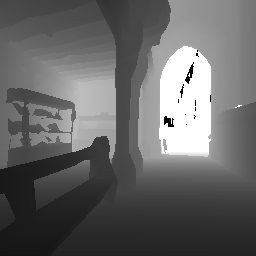
\includegraphics[width=\textwidth]{imagenes/cap5/normalized.png}
    \caption{Imagen normalizada.}
    \end{subfigure}
    \begin{subfigure}[b]{.475\textwidth}
    \centering
    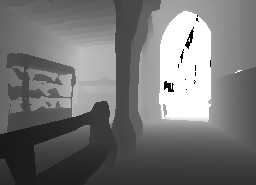
\includegraphics[width=\textwidth]{imagenes/cap5/trimmed.png}
    \caption{Imagen recortada.}
    \end{subfigure}
    
    \begin{subfigure}[b]{.475\textwidth}
    \centering
    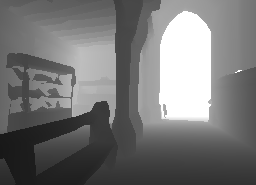
\includegraphics[width=\textwidth]{imagenes/cap5/filled.png}
    \caption{Imagen sin artefactos.}
    \end{subfigure}
    \begin{subfigure}[b]{.475\textwidth}
    \centering
    
\includegraphics[width=\textwidth]{imagenes/cap5/thresholded.png}
    \caption{Imagen con umbral aplicado.}
    \end{subfigure}

	\begin{subfigure}[b]{.475\textwidth}
    \centering
    
\includegraphics[width=\textwidth]{imagenes/cap5/cleaned.png}
    \caption{Imagen sin ruido.}
    \end{subfigure}
    \begin{subfigure}[b]{.475\textwidth}
    \centering
    
\includegraphics[width=\textwidth]{imagenes/cap5/dilated.png}
    \caption{Imagen dilatada.}
    \end{subfigure}

    \caption{Procesamiento realizado sobre la imagen de profundidad.}
    \label{fig:chap5-imageprocess}
\end{figure*}

\subsubsection{Identificación de los obstáculos y la distancia en la imagen}

Tras el preprocesamiento de la imagen, es necesario identificar los obstáculos en la imagen   y estimar la distancia a la que éstos se encuentran. Para eso, se han propuesto dos métodos:

\begin{itemize}
	\item \textbf{Método de contornos:} Este método se basa en la propuesta original de Carlos Sampedro \textit{et al.} \cite{Sampedro2018}. 
	
	La idea principal del método es identificar los contornos que tengan un área mínimo (experimentalmente determinado como $250$ pixeles) en la imagen preprocesada. A partir de estos contornos, se crean máscaras en la imagen original para extraer los obstáculos de nuevo en escala de grises. Finalmente, se obtiene la cercanía de esos obstáculos (a partir del pixel de valor mínimo), usando la siguiente estimación:
	\[distancia = \frac{(pixel\_min / 256) * distancia\_estimada}{umbral\_obstaculo}\]
Donde $pixel\_min$ es el pixel de menor valor en el obstáculo (en el rango ${0, 255}$), $distancia\_estimada$ es un valor heurístico que indica la distancia a la que se encontraría un obstáculo en el umbral (estimado como $2$ metros) y $umbral\_obstaculo$ es el umbral que se ha usado durante la umbralización ($0.15$).

Se puede ver el pseudocódigo del proceso en la Figura \ref{alg:contour}.

\begin{figure}[h]
\begin{algorithm}[H]
\SetAlgorithmName{Algoritmo}{algoritmo}{Lista de algoritmos}
\caption{Identificación de distancias con método de contornos}
\textbf{Variables:} Imagen preprocesada $imagen\_p$, imagen recortada $imagen\_r$, umbral usado durante preprocesamiento $umbral$, distancia estimada hasta el umbral en metros $dist$, área mínima de los contornos en píxeles $area\_min$.\\
\textbf{1.} Inicializa una lista para almacenar las distancias obtenidas, $distancias$.\\
\textbf{2.} Extrae los contornos de la imagen $imagen\_p$ a una lista $contornos$.\\
\textbf{3.} Para cada contorno $cont$ de area $area\_contorno$ en $contornos$, con $area\_contorno \geq area\_min$:\\
\Indp \textbf{3.1.} Aplica una máscara con la forma de $cont$ a $imagen\_r$, obteniendo el obstáculo $obs$ (el obstáculo tal y como está representando en la imágen $imagen\_r$, en escala de grises).\\
\textbf{3.2.} Obtén la distancia mínima en $obs$ (el valor mínimo), $dist\_obs$.\\
\textbf{3.3.} Convierte $dist\_obs$ de un valor entero en el rango $\{0, 255\}$ a una distancia en metros mediante una equivalencia usando $umbral$ y $dist$.\\
\textbf{3.4.} Si $dist\_obs \leq dist$, almacena $dist\_obs$ en $distancias$.\\
\Indm \textbf{4.} Devuelve $distancias$.
\end{algorithm}
\hrule
\caption{Pseudocódigo del método de contornos para identificar distancias a obstáculos.}
\label{alg:contour}
\end{figure}

\newpage 

	\item \textbf{Método de columnas:} Un método original, consistente en dividir la imagen  en columnas de misma anchura, siendo cada columna un posible obstáculo. 
	
	El método consiste en dividir la imagen preprocesada en $8$ (elegido experimentalmente) columnas de anchura idéntica. Tras esto, se cuenta el número de píxeles blancos (obstáculos) en cada columna, considerando las columnas que tengan una cantidad superior al área mínima ($250$ píxeles como se ha mencionado previamente) como obstáculos. Para estas columnas, se estima la distancia a partir de una columna equivalente de la imagen original, usando la fórmula descrita previamente:
	\[distancia = \frac{(pixel\_min / 256) * distancia\_estimada}{umbral\_obstaculo}\]
Donde $pixel\_min$ es el pixel de menor valor en el obstáculo (en el rango ${0, 255}$), $distancia\_estimada$ es un valor heurístico que indica la distancia a la que se encontraría un obstáculo en el umbral (estimado como $2$ metros) y $umbral\_obstaculo$ es el umbral que se ha usado durante la umbralización ($0.15$).

Se puede ver el pseudocódigo del proceso en la Figura \ref{alg:column}.

\begin{figure}[h]
\begin{algorithm}[H]
\SetAlgorithmName{Algoritmo}{algoritmo}{Lista de algoritmos}
\caption{Identificación de distancias con método de columnas}
\textbf{Variables:} Imagen preprocesada $imagen\_p$, imagen recortada $imagen\_r$, umbral usado durante preprocesamiento $umbral$, distancia estimada hasta el umbral en metros $dist$, área mínima de los contornos en píxeles $area\_min$.\\
\textbf{1.} Divide las imágenes $imagen\_p$ y $imagen\_r$ en columnas de anchuras iguales, $columnas\_p$ y $columnas\_r$.\\
\textbf{2.} Para cada columna $col$ con $pixeles$ pixeles blancos en $columnas\_p$ y $col\_r$ en $columnas\_r$, cumpliendo que $pixeles \geq area\_min$:\\
\Indp\textbf{2.1.} Obtén la distancia mínima en $col\_r$ (el valor mínimo), $dist\_obs$.\\
\textbf{2.2.} Convierte $dist\_obs$ de un valor entero en el rango $\{0, 255\}$ a una distancia en metros mediante una equivalencia usando $umbral$ y $dist$.\\
\textbf{2.3.} Si $dist\_obs \leq dist$, almacena $dist\_obs$ en $distancias$.\\
\Indm \textbf{3.} Devuelve $distancias$.
\end{algorithm}
\hrule
\caption{Pseudocódigo del método de columnas para identificar distancias a obstáculos.}
\label{alg:column}
\end{figure}

Este método se propone al considerar que el método anterior daría la misma importancia a un obstáculo grande (que ocupa gran parte de la pantalla) y a uno pequeño siempre y cuando estuviesen a la misma distancia. La idea es remediar ese problema, dando más peso a los obstáculos más grandes. Además, al evitar tener que usar algoritmos de búsqueda de contornos, se espera que la velocidad de ejecución sea mayor.

\end{itemize}

\subsubsection{Cálculo del potencial atractivo y repulsivo}

Tras el cálculo de las distancias a los obstáculos, se calcula el valor de los potenciales atractivos y repulsivos. Este cálculo es equivalente al propuesto por Carlos Sampedro \textit{et al.} \cite{Sampedro2018} originalmente.

El \textbf{potencial atractivo} es la fuerza con la que la meta atrae al agente. Cuanto más cerca esté el agente de la meta, mayor debe ser su influencia. Este potencial se obtiene con la siguiente fórmula:
\[U_{atr} = \alpha p_{goal}(t_r)\]
Donde $\alpha$ es una ganancia positiva usada para aumentar la influencia del potencial (estimada empíricamente como $100$) y $p_{goal}(t_r)$ es la distancia euclídea entre la posición actual del agente y la meta.

El \textbf{potencial repulsivo} es la suma de las fuerzas con las que los obstáculos repelen al agente. Cuantos más obstáculos perciba el agente y más cerca se encuentren, mayor debe ser su influencia. Este potencial se obtiene con la siguiente fórmula:
\[U_{rep} = \beta \sum_{i=1}^{N}(\frac{1}{k+l_i}-\frac{1}{k+l_{max}})\]
Donde $N$ es el número total de obstáculos detectados, $k$ es una constante usada para limitar la influencia de los obstáculos (con valor por defecto $0.04$), $l_i$ es la distancia al obstáculo $i$ en metros, $l_{max}$ es la distancia máxima a la que se detectan los obstáculos (con valor por defecto $2$ metros) y $\beta$ se obtiene con la siguiente fórmula:
\[
\beta = 
\begin{cases}
\delta,& \text{si } p_{goal}(t_r) > d_{infl}\\
\frac{\delta}{exp[4(d_{infl}-p_{goal})]},& \text{si } p_{goal}(t_r) \leq d_{infl}
\end{cases}
\]
Donde $\delta$ es una ganancia positiva usada para aumentar la influencia del potencial (estimada empíricamente como $15$) y $d_{infl}=0.75 l_{max}$ es una distancia a partir de la cual la influencia del potencial repulsivo se disminuye, para fomentar al agente a acercarse a la meta cuando se encuentra próximo a ésta.

Tras el cálculo de ambos potenciales, es posible calcular el \textbf{valor del estado actual}. Cuanto mayor es el valor del estado, mejor estado se considera que es. Este valor se comparará con el valor del estado previo para comprobar si ha mejorado o empeorado, y obtener una recompensa a partir de ello.

Este valor se calcula como:
\[valor_t=-U_{atr}-U_{rep}\]

\subsubsection{Cálculo de la recompensa final}
 
Tras haber calculado los potenciales y el valor del estado, es posible obtener la recompensa final a partir de las siguientes reglas:

\begin{itemize}

\item Si el episodio ha finalizado (ya sea por la acción correspondiente o por limite de acciones) y el agente no está en rango de la meta: \textbf{-100}.

La penalización por finalizar un episodio sin éxito es muy alta para evitar que el agente finalice el episodio antes de tiempo con la intención de evitar penalizaciones por sus acciones.

\item Si el episodio ha finalizado (ya sea por la acción correspondiente o por límite de acciones) y el agente está en rango de la meta: \textbf{+10}.

La recompensa por finalizar un episodio con éxito es menor, pero sigue siendo elevada para fomentar al agente a llegar a la meta y finalizar en ella.

\item En cualquier otro caso:

Si el episodio no ha finalizado tras la acción del agente, se procede a calcular la recompensa a partir de los valores del estado actual y el previo:
\[recompensa = (valor_t - valor_{t-1}) - 0.25, \text{acotado en el rango } [-100, +10]\]

Si el valor del estado alcanzado tras realizar la acción es mayor (la acción lleva a un estado mejor) la recompensa será positiva, mientras que si el valor es menor (la acción lleva a un estado peor) la recompensa será negativa. De esta forma, se fomenta que el agente intente mejorar su posición continuamente.

El término $-0.25$ es una penalización por paso, usada para evitar que el agente permanezca en bucles infinitos sin recompensa y acelerando su progreso.

\end{itemize} 

Una alternativa propuesta es incluir una regla adicional al cálculo de recompensas:
\begin{itemize}
	\item Si el agente ha colisionado con algún obstáculo tras la acción: \textbf{-100} y \textbf{finaliza el episodio}.
	
	Con esta regla adicional, se penaliza notablemente que el agente colisione con los obstáculos, fomentando que evite cualquier colisión con el entorno. Estas colisiones se comprueban usando la métrica \textit{COLLISIONS}.
\end{itemize}

\newpage

\section{Arquitectura del agente}

En esta sección se discuten las arquitecturas (redes neuronales) propuestas para el agente, su funcionamiento y su implementación. Se han propuesto dos arquitecturas, de las cuales se ha elegido una finalmente:

\begin{itemize}
		\item Una primera aproximación basada en \textbf{redes neuronales convolucionales}.
		\item Una segunda aproximación basada en un \textbf{enfoque mixto}, con redes convolucionales y redes neuronales densas tradicionales.
\end{itemize}

\subsection{Propuesta 1: Red convolucional (CNN)}

La primera aproximación está basada en el uso de \textbf{redes convolucionales \textit{(CNNs)}} para el procesamiento de la imagen, extrayendo las características profundas relevantes para trabajar posteriormente con ellas. 

Ahora bien, los valores numéricos (parte del estado a procesar) no pueden ser usados directamente por las capas de convolución. Para solventar esto, los dos valores numéricos (distancia y ángulo) son concatenados directamente a la salida aplanada de las convoluciones, para ser procesados posteriormente por las capas densas de neuronas.

La arquitectura de la red neuronal se ha basado en la arquitectura original de \textit{AlexNet} \cite{Krizhevsky2012ImageNetCW}, adaptada de forma \textit{ad-hoc} para las necesidades del trabajo y las limitaciones existentes de memoria y tiempo.

La red se puede dividir en varias secciones consecutivas:
\begin{enumerate}
	\item \textbf{Entrada:} La entrada se obtiene de una muestra del \textit{Experience Replay}. Cada elemento de esta muestra es un estado, correspondiendose con la definición dada previamente de estado:
	\begin{itemize}
		\item Una imagen de profundidad (escala de grises), en forma de una matriz bidimensional de tamaño $256x256$ con una única capa.
		\item Dos valores escalares: la distancia y el ángulo hasta la meta.
	\end{itemize}
	
	\item \textbf{Convolución:} El primer paso de la red es procesar la imagen a través de varios procesos de convolución, con el fin de obtener las características profundas de ésta. Para esto, se tienen \textbf{tres} procesos de convolución consecutivos, cada uno de ellos formado por, en orden:
		\begin{itemize}
			\item Capa convolucional bidimensional de 16 filtros. El tamaño del \textit{kernel} es de $5x5$, $3x3$ y $3x3$ en cada proceso respectivamente.
			\item Función de activación ReLU.
			\item Capa de \textit{pooling} por función de máximo. El tamaño del \textit{pooling} es de $3x3$, $3x3$ y $2x2$ en cada proceso respectivamente.
		\end{itemize}
		
	A pesar de ser típico en redes convolucionales, no se ha incluido ninguna capa de \textit{batch normalization} durante el proceso de convolución. Ésto se debe a que el proceso de normalización introduce ruido que puede alterar el proceso de aprendizaje por refuerzo \cite{Salimans2016}.
	
	\item \textbf{Aplanado (\textit{Flatten}):} Tras la convolución de la imagen, el resultado del proceso (una matriz tridimensional profunda con las características de la imagen) es aplanado a un conjunto unidimensional de neuronas. Esto permite a las capas posteriores trabajar con la información obtenida. Esta capa no cuenta con ninguna función de activación.
	
	En este paso además se concatenan los dos valores escalares de la entrada (distancia y ángulo a la meta). Estos valores no han sido incluidos previamente al no poder ser procesados por las capas convolucionales. Al añadirlos ahora, las capas posteriores podrán trabajar con la información.
	
	\item \textbf{Capas densas:} Tras el aplanamiento y concatenación de la información en el paso previo, se incluyen \textbf{dos} capas densas (capas de neuronas totalmente conectadas) para extraer relaciones entre la información obtenida.
	
	Estas capas densas cuentan con $256$ neuronas cada una, utilizando \textit{ReLU} como función de activación.
	
	\item \textbf{Salida:} Finalmente, la capa de salida es una capa densa de cuatro neuronas, donde cada neurona se corresponde con el valor Q de una de las cuatro acciones disponibles para el agente. Estas neuronas cuentan con función de activación lineal.
\end{enumerate}

Se puede observar un esquema de la arquitectura en la Figura \ref{fig:chap5-arc1}.

\begin{figure}
    \centering
    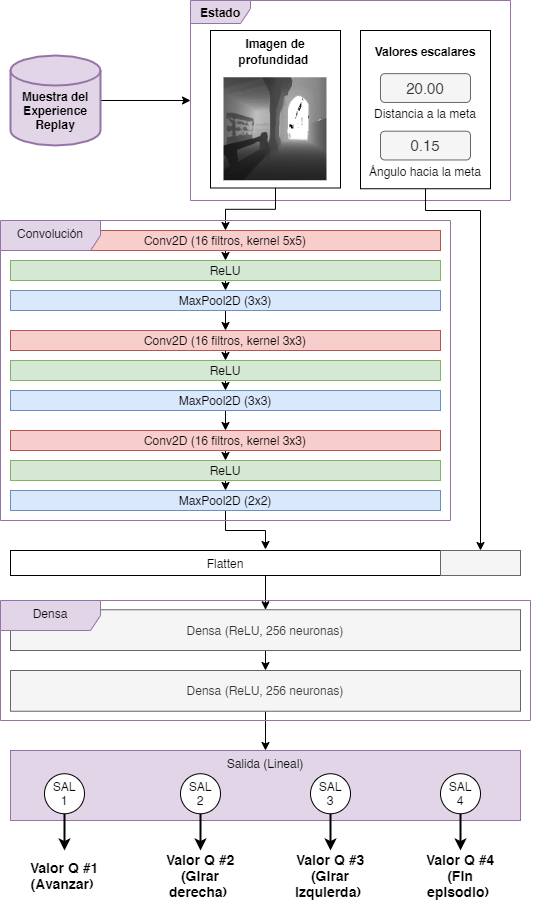
\includegraphics[height=0.95\textheight]{imagenes/cap5/arquitectura1.png}
    \caption{Arquitectura de la red neuronal - Propuesta 1 (CNN).}
    \label{fig:chap5-arc1}
\end{figure}	

La red neuronal ha sido implementada utilizando las librerías \textit{TensorFlow} y \textit{Keras}. Para las funciones usadas por la red para su entrenamiento, se ha optado por utilizar algunos algoritmos tradicionalmente usados en problemas de aprendizaje profundo, siendo éstos:
\begin{itemize}
	\item \textbf{Función de inicialización de pesos:} Glorot y Bengio \cite{Glorot2010UnderstandingTD}.
	\item \textbf{Función de optimización:} Adam \cite{adam2014}.
	\item \textbf{Función de error:} Error cuadrático medio. Esta función de error es usada tradicionalmente en problemas de aprendizaje por refuerzo profundo.
\end{itemize}

Tras realizar pruebas iniciales (entrenamientos cortos) con la arquitectura propuesta, se observaron una serie de problemas con ésta:

\begin{itemize}
	\item \textbf{Ineficiencia en memoria:} Debido al tamaño de la red y a problemas con la librería utilizada, el uso de memoria (tanto memoria \textit{RAM} del ordenador como de la \textit{GPU}) era excesivo. Además, este uso crecía tras cada episodio hasta llegar a un punto en el que se detenía el entrenamiento por falta de memoria.
	
	Esto provocaba que no fuese posible realizar entrenamientos largos, y que los entrenamientos realizados fuesen notablemente más lentos de lo esperado.
	\item \textbf{Malos resultados:} Durante el proceso de entrenamiento se observó que los resultados obtenidos por la red eran peores de lo que se podría esperar, sin mostrar signos de aprendizaje. Esto se puede deber al uso de los valores escalares, al ser menos relevantes (2 neuronas) frente a la información obtenida de la imagen (miles de neuronas).
\end{itemize}

Por estos problemas, se ha optado por \textbf{descartar} esta arquitectura en favor de la segunda propuesta, descrita a continuación. La implementación de esta propuesta se conserva en los ficheros \textit{models/DEPRECATED{\_}reactive{\_}navigation{\_}keras.py} y \textit{trainers/DEPRECATED{\_}reactive{\_}navigation{\_}trainer{\_}keras.py}, por motivos de documentación

\subsection{Propuesta 2: Red mixta (CNN + MLP)}

La segunda aproximación está basada en el uso de \textbf{redes híbridas} (es decir, redes formadas por varias redes neuronales más pequeñas).

Una red convolucional no está preparada para trabajar con valores escalares numéricos. Ahora bien, un perceptrón multicapa (\textit{MLP}) estándar no puede procesar imágenes con el mismo rendimiento que una red convolucional. Por tanto, una de las mejores opciones para trabajar con entradas mixtas de imágenes y valores escalares es procesar cada tipo de entrada en una red neuronal separada específica (las imágenes en redes convolucionales y los valores escalares en redes densas), obteniendo resultados que serán juntados y procesados posteriormente en una red neuronal final.

La arquitectura de esta propuesta está inspirada por las arquitecturas propuestas para resolver otros problemas con entrada mixta de imágenes y valores numéricos, como el trabajo de Md Manjurul Ahsan \textit{et al.}  para distinguir casos de COVID-19 \cite{sym12091526} o el trabajo de Yanyu Zhang aplicando redes mixtas al aprendizaje por refuerzo profundo \cite{DBLP:journals/corr/abs-2010-00717}. Se ha desarrollado la arquitectura de forma \textit{ad-hoc} para las necesidades del proyecto.

La propuesta consta con dos redes neuronales (una red convolucional y un perceptrón multicapa) que procesan sus entradas de forma paralela. Tras esto, las salidas de ambas redes se pasan a una red final que obtiene el resultado. La arquitectura de las tres redes son las siguientes:

\begin{itemize}

\item \textbf{Red convolucional (CNN):} Esta red se encarga del procesamiento de la imagen de profundidad de la entrada, extrayendo las características profundas de ésta para ser aprovechadas posteriormente. Consta de las siguientes capas:
\begin{enumerate}
	\item \textbf{Entrada:} La entrada es una imagen de profundidad (escala de grises) en forma de matriz bidimensional de tamaño $256x256$, con una única capa. Esta imagen se obtiene de los estados muestreados del \textit{Experience Replay}.
	\item \textbf{Convolución:} El primer paso de la red es procesar la imagen para extraer las características principales, reduciendo su tamaño. Para esto se usan \textbf{tres} procesos de convolución consecutivos, cada uno de ellos formado por, en orden:
	\begin{itemize}
		\item Capa convolucional bidimensional. El número de filtros depende del proceso de convolución, siendo éste de $16$, $32$ y $16$ filtros respectivamente. El tamaño del $kernel$ también varía dependiendo del proceso, siendo éste de $5x5$, $3x3$ y $3x3$ en cada proceso respectivamente.
		\item Función de activación ReLU.
		\item Capa de \textit{pooling} con función de máximo. El tamaño de \textit{pooling} es de $3x3$, $3x3$ y $2x2$ respectivamente dependiendo del proceso de convolución.
	\end{itemize}
	\item \textbf{Aplanado (\textit{Flatten}):} Tras la convolución de la imagen, es necesario aplanar el resultado (la matriz tridimensional con las características identificadas) a un conjunto unidimensional de neuronas. Este aplanamiento permite a las capas densas posteriores trabajar de forma correcta con la información. Esta capa no cuenta con ninguna función de activación.
	\item \textbf{Capa densa:} En este caso, tras el aplanado hay una única capa densa (capa de neuronas totalmente conectadas) de \textbf{64} neuronas usando \textbf{ReLU} como función de activación. Con esta capa se busca identificar relaciones existentes entre las características encontradas previamente con la convolución.
	\item \textbf{Salida:} La capa de salida es una única capa densa con tres neuronas, con función de activación lineal. Se ha optado por utilizar una función de activación lineal para no modificar el valor de salida alcanzado de ninguna manera, buscando evitar sesgos.
	
	Estas neuronas posteriormente servirán como entrada para otra red neuronal.
\end{enumerate}

\item \textbf{Red neuronal profunda / Perceptrón multicapa (MLP):} Esta red se encarga del procesamiento de los valores numéricos de la entrada, preparándolos para su uso posterior. Consta de las siguientes capas:

\begin{enumerate}
\item \textbf{Entrada:} La entrada son dos valores numéricos (la distancia y el ángulo hacia la meta), obtenidos de los estados muestreados del \textit{Experience Replay}.
\item \textbf{Capas ocultas:} Tras la entrada, la red cuenta con \textbf{dos} capas densas (neuronas totalmente conectadas) de \textbf{diez} neuronas cada una, con función de activación ReLU. Estas capas de neuronas se encargan de procesar las entradas numéricas.

El número de neuronas se ha obtenido a partir del número de entradas y salidas, siendo $2(entrada + salida) = 10$.
\item \textbf{Salida:} La capa de salida es una única capa densa con tres neuronas, con función de activación lineal. De nuevo, se utiliza una función de activación lineal para que el valor de las neuronas de salida no se vea modificado de ninguna forma.

Estas neuronas serán usadas posteriormente como entrada para otra red neuronal.
\end{enumerate}

\item \textbf{Red mixta (CNN + MLP):} Esta red toma las salidas de las dos redes anteriores, juntándolas y procesándolas para obtener las salidas finales de la red neuronal. La arquitectura de esta red es una red neuronal estándar, con las siguientes capas:
\begin{enumerate}
\item \textbf{Concatenación / Entrada:} La entrada de la red es una concatenación de las salidas de las dos redes neuronales anteriores: \textbf{3} neuronas de la imagen procesada y \textbf{3} neuronas de los valores numéricos procesados, para un total de \textbf{6} neuronas. Esta capa no tiene ninguna función de activación.

Se ha decidido que ambas redes neuronales tengan el mismo número de neuronas en la salida para que ambas partes del estado (imagen y valores numéricos) tuviesen la misma relevancia a la hora de obtener una salida. Además, se ha elegido usar \textbf{tres} neuronas en cada salida por tener un número pequeño de neuronas, pero suficientemente grande para que haya una expresión rica de características.
\item \textbf{Capas ocultas:} Tras la entrada, la red cuenta con \textbf{dos} capas densas de \textbf{32} neuronas, con funciones de activación ReLU.

Se ha optado por utilizar dos capas con un número moderado de neuronas frente a una capa con una gran cantidad de neuronas por ofrecer mejor rendimiento, dando la posibilidad con más capas de encontrar más relaciones entre datos.
\item \textbf{Salida:} La capa de salida es una capa densa de cuatro neuronas, donde cada neurona se corresponde con el valor Q de una de las cuatro acciones disponibles para el agente. Esta capa utiliza una función de activación lineal.
\end{enumerate}

\end{itemize}

Se puede observar un esquema de la arquitectura en la Figura \ref{fig:chap5-arc2}.

\begin{figure}
    \centering
    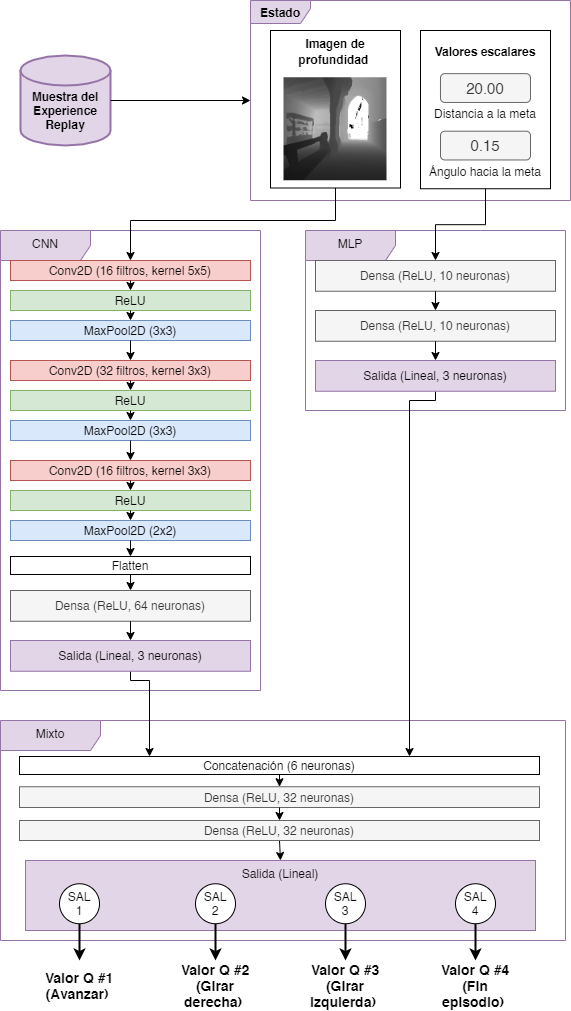
\includegraphics[height=0.95\textheight]{imagenes/cap5/arquitectura2.png}
    \caption{Arquitectura de la red neuronal - Propuesta 2 (Mixta).}
    \label{fig:chap5-arc2}
\end{figure}	

A diferencia de la propuesta anterior, la red neuronal ha sido implementada utilizando la librería \textit{PyTorch}, estando disponible la implementación en el fichero \textit{models/reactive{\_}navigation.py}. Para las funciones usadas por la red durante su entrenamiento, se han usado algoritmos más novedosos que los de la propuesta anterior, siendo estos:

\begin{itemize}
	\item \textbf{Función de inicialización de pesos:} Kaiming \cite{DBLP:journals/corr/HeZR015}.
	\item \textbf{Función de optimización:} Adam \cite{adam2014}.
	\item \textbf{Función de error:} Error de Huber \cite{10.1214/aoms/1177703732}. 
	
	Esta función es una variante del error cuadrático medio propuesta por Huber en 1964, siendo más resistente a los valores aislados. Concretamente, la función es cuadrática para valores residuales pequeños, mientras que se vuelve lineal para valores elevados.
\end{itemize}

Esta propuesta ha sido elegida como la arquitectura definitiva usada por el agente, al ofrecer mejores resultados en un tiempo de entrenamiento menor, sin ningún error ni problema durante la ejecución.

\section{Actuación del agente}

El proceso de actuación del agente está basado en el proceso de actuación estándar de un agente de \textit{Deep Q-Learning} siguiendo el paradigma de exploración / explotación, pudiendo ser observado en la Figura \ref{alg:act}.

\begin{figure}[h]
\begin{algorithm}[H]
\SetAlgorithmName{Algoritmo}{algoritmo}{Lista de algoritmos}
\caption{Actuación del agente}
\textbf{Entradas:} Estado $s$, formado por una imagen de profundidad $depth$ y dos valores numéricos, la distancia a la meta $dist$ y  el ángulo hacia la meta $angle$.\\
\textbf{Variables internas del agente:} Probabilidad de acción aleatoria $\epsilon$, lista de acciones posibles $action\_list$.
 el agente conserva una variable $\epsilon$ para el ratio de exploración / explotación.\\
\textbf{1.} Genera un valor aleatorio $rand$ en el rango $[0.0, 1.0]$.\\
\textbf{2.} Si $rand < \epsilon$:\\
\Indp \textbf{2.1} Exploración. Se elige una acción $action$ de $action\_list$ aleatoriamente, siguiendo una distribución uniforme.\\
\Indm \textbf{3.} En otro caso ($rand \geq \epsilon$):\\
\Indp \textbf{3.1.} Explotación. Procesa el estado $s$ a través de la red neuronal, obteniendo la lista de valores Q para cada par estado-acción $q\_values$.\\
\textbf{3.2.} Elige la acción $action$ de $action\_list$ que tenga el máximo valor en $q\_values$.\\
\Indm \textbf{4.} Devuelve $action$.
\end{algorithm}
\hrule
\caption{Proceso de actuación del agente.}
\label{alg:act}
\end{figure}

Como ya se ha mencionado, la actuación del agente sigue el paradigma de exploración-explotación, usando $\epsilon$ como la variable que regula el proceso. $\epsilon$ se actualiza durante el entrenamiento tras cada episodio siguiendo la siguiente fórmula:
\[\epsilon= max\left( \frac{(\epsilon_{init} - \epsilon_{min}) * porcentaje}{\epsilon_{min\_porcentaje}} - \epsilon_{init}, \epsilon_{min} \right)\]
Donde $\epsilon_{init}$ es el valor inicial de $\epsilon$ (por defecto $1.0$), $\epsilon_{min}$ es el valor mínimo alcanzado por $\epsilon$ (por defecto $0.05$), $\epsilon_{min\_porcentaje}$ es el porcentaje de episodios tras el cual el valor de $\epsilon$ alcanzará $\epsilon_{min}$ (por defecto $0.8$, el $80\%$ de los episodios) y $porcentaje$ es el porcentaje actual de episodios completados.

En esencia, el valor de $\epsilon$ decrece linealmente desde su valor inicial, $\epsilon_{init}$, hasta su valor final, $\epsilon_{min}$, conforme el agente completa episodios. El valor final será alcanzado tras completar el $\epsilon_{min\_porcentaje}\%$ de los episodios (por ejemplo, para un entrenamiento de 10.000 episodios $\epsilon_{min}$ se alcanzaría a los 8000 episodios). El valor de $\epsilon$ no puede bajar de $\epsilon_{min}$ en ningún momento.

El objetivo es que en los primeros episodios el agente explore una gran cantidad de estados (\textbf{exploración}) mientras no tiene suficiente conocimiento como para tener una política de acciones de calidad. Conforme el agente completa episodios y adquiere conocimiento, se busca que éste empiece a aprovechar las experiencias previas en los episodios finales (\textbf{explotación}), efectuando menos acciones aleatorias y más acciones acordes a la política aprendida.

Cuando el agente es usado fuera de un entorno de entrenamiento (como puede ser durante su evaluación), el valor de $\epsilon$ se queda fijado como $\epsilon=0$, para explotar totalmente la política sin ninguna acción aleatoria.

\section{Entrenamiento del agente}

En esta sección se describe el proceso seguido por el agente para realizar su entrenamiento. El agente ha sido entrenado utilizando el algoritmo de \textit{Deep Q-Learning}, siendo el pseudocódigo del algoritmo el expuesto en la Figura \ref{alg:chap5-dql}.

\begin{figure}[h]
\begin{algorithm}[H]
\SetAlgorithmName{Algoritmo}{algoritmo}{Lista de algoritmos}
\caption{Entrenamiento del agente}
\textbf{Variables iniciales:} Dos agentes, un agente conteniendo la red Q, $agente\_q$, y un agente conteniendo la red objetivo, $agente\_obj$. \textit{Experience Replay} $exp\_replay$ donde se almacenan las experiencias del agente. Número total de episodios a realizar durante el entrenamiento, $ep\_total$. $\epsilon$, probabilidad de realizar una acción aleatoria.\\
\textbf{1.} Inicializa un contador, $cont\_ep=0$, para almacenar el numero de episodios realizados hasta el momento.\\
\textbf{2.} Mientras $cont\_ep < ep\_total$:\\
\Indp \textbf{2.1} Inicializa el episodio $episodio$, obteniendo el estado inicial $estado$.\\
\textbf{2.2} Mientras $episodio$ no haya finalizado:\\
\Indp \textbf{2.2.1.} $agente\_q$ elige la acción $accion$ a realizar para $estado$ dependiendo de $\epsilon$, usando el método descrito previamente.\\
\textbf{2.2.2.} Se aplica $accion$ a $estado$, obteniendo una recompensa $recompensa$, un nuevo estado $n\_estado$ y un indicador de si $n\_estado$ es final, $final$.\\
\textbf{2.2.3.} Se almacena $estado$, $accion$, $recompensa$, $n\_estado$ y $final$ en $exp\_replay$.\\
\textbf{2.2.4.} Se toma una muestra $batch$ de $exp\_replay$, y se entrena al agente $agente\_q$ a partir de $batch$, usando los resultados de $agente\_q$ y $agente\_obj$.\\
\textbf{2.2.5.} $estado=n\_estado$.\\
\Indm \textbf{2.3.} Actualiza $agente\_obj$ con los pesos de $agente\_q$.\\
\textbf{2.4.} Actualiza $\epsilon$.\\
\textbf{2.5.} $cont\_ep++$.\\
\textbf{2.6.} Documenta el proceso de entrenamiento.\\
\Indm \textbf{3.} Devuelve los pesos de $agente\_q$ como agente entrenado.
\end{algorithm}
\hrule
\caption{Proceso de entrenamiento del agente.}
\label{alg:chap5-dql}
\end{figure}

Se ha optado por utilizar \textit{Deep Q-Learning} frente a otras técnicas de aprendizaje por refuerzo profundo como \textit{PPO} principalmente por familiaridad con la técnica. Además, \textit{Deep Q-Learning} sigue ofreciendo buenos resultados en problemas de aprendizaje por refuerzo profundo, especialmente si se aplican mejoras como \textit{Prioritized Experience Replay}.

Se han planteado dos variantes para el entrenamiento, dependiendo de la técnica utilizada:
\begin{itemize}
	\item Entrenamiento usando \textit{Deep Q-Learning} estándar.
	\item Entrenamiento usando \textit{Deep Q-Learning} con \textit{Prioritized Experience Replay}.
\end{itemize}

A continuación, se describen los elementos principales del entrenamiento.

\subsection{\textit{Replay Memory} y memorización de la experiencia}

El \textit{Replay Memory} del agente se encarga de almacenar las experiencias previas del agente, para su muestreo posterior durante el entrenamiento. Estas experiencias son almacenadas con la forma $<s, a, r, s', f>$, siendo cada elemento:

\begin{itemize}
\item $s$: Estado inicial de la experiencia.
\item $a$: Acción aplicada sobre el estado $s$.
\item $r$: Recompensa obtenida tras aplicar la acción $a$ al estado $s$.
\item $s'$: Estado nuevo, alcanzado tras aplicar la acción $a$ al estado $s$.
\item $f$: Valor booleano que indica si $s'$ es un estado final (ha provocado el final del episodio) o no.
\end{itemize}

Internamente, el \textit{Replay Memory} es una cola FIFO estándar de tamaño $M$ (por defecto, $20000$ posiciones) donde se introducen las experiencias. Cuando la cola se llena, la introducción de una nueva experiencia provocará que la experiencia más antigua sea eliminada. De esta forma, se evita que el conocimiento del agente se estanque al ir renovando las experiencias conforme se van experimentando nuevas experiencias.

Tras cada actuación del agente, se introduce la experiencia (los valores descritos anteriormente) en la memoria y se realiza un proceso de aprendizaje como se verá posteriormente.

La variante usando \textit{Prioritized Experience Replay} presenta las siguientes diferencias:
\begin{itemize}
\item El \textit{Replay Memory} pasa de almacenar directamente la experiencia $<s, a, r, s', f>$ a una tupla $(experiencia, error)$. En esta tupla, $experiencia$ sigue teniendo la estructura $<s, a, r, s', f>$, pero $error$ simboliza el error que presenta la experiencia (siendo éste la diferencia entre los valores Q que se espera que devuelva la red para $s$ y los valores Q realmente obtenidos).
\item Cuando se inserta una experiencia en el \textit{Replay Memory}, se inserta inicialmente como $(experiencia, \infty)$ (es decir, un valor de error infinito). Esto se debe a que inicialmente no se conoce el error, por lo que se busca el error más alto posible para fomentar que el agente aprenda la experiencia.
\end{itemize}

\subsection{Aprendizaje a partir de las experiencias}

Tras la memorización de una experiencia, se realiza aprendizaje a partir de una muestra tomada del \textit{Experience Replay}, viéndose el proceso general en la Figura \ref{alg:chap5-apst}.

\begin{figure}
\begin{algorithm}[H]
\SetAlgorithmName{Algoritmo}{algoritmo}{Lista de algoritmos}
\caption{Aprendizaje a partir de la experiencia (estándar)}
\textbf{Variables iniciales:} \textit{Experience Replay} $exp\_replay$. Dos agentes, el agente con la red neuronal Q $agente\_q$ y el agente con la red neuronal objetivo $agente\_obj$. $\gamma$, el peso dado a las nuevas experiencias en \textit{Deep Q-Learning}.\\
\textbf{1.} Obtén una muestra $muestra$ de $exp\_replay$, de tamaño $M$. Si $tamaño(exp\_replay) < M$ \textbf{finaliza el proceso sin aprender.}\\
\textbf{2.} Obtén los valores Q $Q\_s$ para los estados actuales contenidos en $M$ usando al agente Q $agente\_q$.\\
\textbf{3.} Obtén los valores Q $Q\_s'$ para los estados alcanzados contenidos en $M$ usando al agente objetivo $agente\_obj$.\\
\textbf{4.} Para cada experiencia $exp$ de la muestra $M$, donde $exp\_a$ es la acción tomada en $exp$, $exp\_r$ es la recompensa obtenida en $exp$, $exp\_f$ es la indicación de si $exp$ fue final y $exp\_q$ y $exp\_q'$ son los valores Q para el estado actual y alcanzado de $exp$ (calculados previamente en $Q\_s$ y $Q\_s'$ respectivamente):\\
\Indp \textbf{4.1.} Actualiza el valor Q asociado a la acción $exp\_a$ en $exp\_s$ siguiendo la siguiente fórmula:
\[
exp\_q(exp\_a)=
\begin{cases}
	exp\_r,& \text{si } exp\_f \text{ (si la experiencia es final)}\\
	exp\_r + \gamma * max(exp\_q'),& \text{en cualquier otro caso}\\
\end{cases}
\]\\
\Indm \textbf{5.} Actualiza las predicciones de $agente\_q$ para los estados actuales de $M$ usando las nuevas predicciones $exp\_q$ (usando retropropagación).\\
\end{algorithm}
\hrule
\caption{Proceso de aprendizaje a partir de las experiencias (estándar).}
\label{alg:chap5-apst}
\end{figure}

Hay algunos detalles importantes que remarcar sobre el proceso:
\begin{itemize}
	\item Por defecto, el tamaño de la muestra es de $64 experiencias$. Se ha optado por no entrenar al agente hasta que el \textit{Replay Memory} contenga al menos 64 experiencias, como en la propuesta original de \textit{Deep Q Learning}, para evitar problemas con la subdivisión de las muestras (como se verá a continuación).
	\item El aprendizaje se realiza en \textit{batch} (en paralelo). Esto significa que todas las muestras son pasadas a través de la red neuronal de forma simultanea, aprovechando el paralelismo ofrecido por las GPUs y mejorando el rendimiento.
	\item Para mejorar el uso en memoria, cada muestra se divide en submuestras de menor tamaño (por defecto, muestras de $64$ experiencias se dividen en submuestras de $32$ experiencias), que son pasadas consecutivamente por la red neuronal.
	
	Esto se ha hecho para suplir los problemas de memoria que surgieron durante el entrenamiento (al no haber suficiente memoria para procesar todos los valores a través de la red neuronal al mismo tiempo), haciendo más eficiente el uso de memoria a costa del tiempo de entrenamiento. Aun así, el rendimiento es notablemente superior al de un entrenamiento no paralelo.
\end{itemize}

La variante usando \textit{Prioritized Experience Replay} presenta las siguientes diferencias respecto a la Figura \ref{alg:chap5-apst}:
\begin{itemize}
\item El muestreo de experiencias no sigue una distribución uniforme, sino que sigue la siguiente distribución, siendo la probabilidad de elegir una experiencia $i$:
\[P(i)=\frac{p_i^{\alpha}}{\sum_k p_k^{\alpha}}\]
Donde $p_i$ es la prioridad de la experiencia $i$ (siendo $p_i=\frac{1}{rango(i)}$, donde $rango(i)$ es la posición de la experiencia $i$ en el \textit{Replay Memory} si éste se ordena de mayor a menor error) y $\alpha$ es una constante que indica el el grado de priorización (por defecto $0.5$).

Esto significa que las experiencias con mayor error tienen más probabilidad de ser muestreadas.
\item Los valores Q actualizados son normalizados con un peso $w_i$, siendo el peso de la experiencia $i$:
\[w_i=\left(\frac{1}{N} \frac{1}{P(i)}\right)^{\beta}\]
Donde $N$ es el número total de experiencias en el \textit{Replay Memory} y $\beta$ es un factor para ajustar la influencia del peso (por defecto $0.5$).

Por tanto, la actualización de valores Q en el punto \textbf{4.1} pasa a ser:
\[
exp\_q(exp\_a)=
\begin{cases}
	exp\_r * w_i,& \text{si } exp\_f \text{ (si la experiencia es final)}\\
	(exp\_r + \gamma * max(exp\_q')) * w_i,& \text{en cualquier otro caso}\\
\end{cases}
\]
\item Tras la actualización de los pesos de la red neuronal Q, los errores de las experiencias muestreadas del \textit{Replay Memory} son actualizados. Estos errores son calculados usando el error cuadrático medio, siendo la fórmula:
\[error=(q\_esperado - q\_obtenido)^2\]
\end{itemize}

\subsection{Documentación del entrenamiento}

Al final de cada episodio, el agente documenta el progreso durante el entrenamiento, imprimiendo en un fichero las siguientes métricas:
\begin{itemize}
	\item ID del episodio.
	\item Duración del episodio (en segundos).
	\item Número de acciones realizadas durante el episodio.
	\item Distancia inicial y final hasta la meta.
	\item Distancia recorrida hasta la meta ($dist\_inicial - dist\_final$). Este valor puede ser negativo si la posición final del agente es más lejana que la inicial.
	\item Exitoso (\textbf{Verdadero} si el agente ha alcanzado la meta, \textbf{Falso} en cualquier otro caso).
	\item Recompensa media obtenida.
\end{itemize}

A partir de estas métricas se realizará un análisis del rendimiento del agente durante el entrenamiento en el Capítulo 6.

Además, el agente almacena registros de su progreso durante el entrenamiento (\textit{checkpoints}), almacenando un total de \textbf{100} \textit{checkpoints} a lo largo de todo el entrenamiento (aproximadamente uno cada 150 episodios). Estos \textit{checkpoints} (ficheros de formato \textit{.pt}) contienen la siguiente información:
\begin{itemize}
	\item Los pesos de la red neuronal objetivo.
	\item El fichero de configuración que se estaba utilizando durante el entrenamiento.
\end{itemize}

A partir de estos \textit{checkpoints} es posible reanudar el entrenamiento en cualquier momento, y usarlos como los pesos finales para el agente entrenado.

\chapter{Experimentación}

\section{Detalles de la experimentación}

\subsection{Parametros utilizados}
[EXPERIMENTOS A REALIZAR, PARAMETROS A USAR, ORDENADOR USADO, ETC]
[PARA REPRODUCIBILIDAD VAMOS]

\subsection{Experimentos realizados}

\section{Resultados obtenidos}

\subsection{Elección del conjunto de datos}

\subsection{Agentes con \textit{Deep Q-Learning} estándar}

\subsection{Agentes con \textit{Deep Q-Learning} priorizado}

\section{Comparativa y análisis de resultados}

\subsection{Comparativa durante el entrenamiento}

\subsection{Comparativa de los agentes entrenados}
[TASA DE EXITO, CUAL ES MEJOR, ETC]

\subsection{Análisis de los resultados}

\chapter{Conclusiones}

\section{Conclusiones}

\section{Trabajo futuro}

PLANTEAMIENTO EXTRA: AGENTE INFORMADO DURANTE ENTRENAMIENTO

%------------------------------------------------
%% Bibliografia:

\addcontentsline{toc}{chapter}{Bibliografía}
\printbibliography

%%-----------------------------------------------
%% Anexos
\appendix
\clearpage 
\addcontentsline{toc}{chapter}{Anexos}
\chapter{Manual de usuario}
[NO TENGO MUY CLARO COMO SE ESCRIBIAN LOS APENDICES NO TE VOY A ENGAÑAR]
[EN LATEX ME REFIERO]

[APENDICES PROBABLES:]
[MANUAL DE USUARIO, COMO GENERO GRAFICAS, CONTENIDOS DEL CD]









 

\chapter{Ficheros de configuración}

Este anexo contiene los ficheros de configuración desarrollados durante el trabajo. En total, se han desarrollado un total de \textbf{12} ficheros de configuración, aunque se pueden dividir en \textbf{4} tipos básicos:

\begin{itemize}
	\item \textbf{Fichero base:} Este fichero contiene la configuración básica y sirve de base para el resto de ficheros (siendo importados por éstos)
	\item \textbf{Ficheros de entrenamiento:} Este fichero contiene la configuración necesaria para el entrenamiento de los agentes, incluyendo los parámetros usados durante \textit{Deep Q-Learning}. Hay \textbf{8} variantes de este fichero dependiendo de la combinación de variantes a utilizar.
	\item \textbf{Ficheros de \textit{benchmark}:} Este fichero contiene la configuración usada para la evaluación de los agentes. Hay \textbf{2} variantes de este fichero, dependiendo del conjunto de datos a usar (\textit{Matterport3D} o \textit{Gibson}).
	\item \textbf{Fichero de generación de video:} Este fichero contiene la configuración usada para generar video del agente durante un episodio. Contiene un bloque con una clave \textit{dummy} de \textit{RL} para poder usar las utilidades de generación de video de \textit{Habitat}.
\end{itemize}

Los ficheros creados (junto a su documentación en inglés) se muestran a continuación.

\section{Fichero base}

\begin{lstlisting}[language=yaml]
# REACTIVE NAVIGATION
# General evaluation / showcase configuration
# Developed by Luna Jimenez Fernandez
#
# This file contains all general parameters to be used while evaluating 
# or showcasing the trained agents.
# 
# In addition, the contents of this file are also used as a basis for the configuration
# used while training the agents. Training specific parameters can be found in the 
# method-specific files (such as reactive_pointnav_train.yaml)
#
# Finally, some of the parameters are specified via arguments during program launch:
#	- Agent type
#	- Dataset and splits to be used
#	- Path to pre-trained weights
#

ENVIRONMENT:
  MAX_EPISODE_STEPS: 1000

SIMULATOR:
  AGENT_0:
    SENSORS: ['RGB_SENSOR', 'DEPTH_SENSOR']
  RGB_SENSOR:
    WIDTH: 256
    HEIGHT: 256
  DEPTH_SENSOR:
    WIDTH: 256
    HEIGHT: 256
    
  # Physics are explicitely disabled, to avoid segmentation faults
  HABITAT_SIM_V0:
    ENABLE_PHYSICS: False
    # PHYSICS_CONFIG_FILE: "None"
    

# DATASET: Data path, split and name are specified via argument
DATASET:
  TYPE: PointNav-v1
#  SPLIT: 
#  DATA_PATH:
#  NAME:

TASK:
  TYPE: Nav-v0
  SUCCESS_DISTANCE: 0.3
  SENSORS: ['POINTGOAL_WITH_GPS_COMPASS_SENSOR']
  POSSIBLE_ACTIONS: ['STOP', 'MOVE_FORWARD', 'TURN_LEFT', 'TURN_RIGHT']
  POINTGOAL_WITH_GPS_COMPASS_SENSOR:
    GOAL_FORMAT: "POLAR"
    DIMENSIONALITY: 2
  GOAL_SENSOR_UUID: pointgoal_with_gps_compass
  MEASUREMENTS: ['DISTANCE_TO_GOAL', 'SUCCESS', 'SPL', 'SOFT_SPL', 'COLLISIONS']
  SUCCESS:
    SUCCESS_DISTANCE: 0.3
\end{lstlisting}

\section{Ficheros de entrenamiento}

\begin{lstlisting}[language=yaml]
# REACTIVE NAVIGATION
# Reactive Navigation Agent training configuration
# Developed by Luna Jimenez Fernandez
#
# This file contains all the specific parameters used by the agent training, including
# both the Deep Q Learning and the Reward computation parameters
#
# Note that this config is added on top of "base_config.yaml", so both files need to be configured
# The following arguments can be found in "base_config.yaml":
#	- Steps per episode (ENVIRONMENT->MAX_EPISODE_STEPS)
#	- Goal radius (TASK->SUCCESS_DISTANCE)
#
# NOTE: Not all parameters are configured via config, the following parameters can be specified
# as arguments when launching the script:
#	- Agent type
#	- Dataset and splits to be used
#	- Path to pre-trained weights
#

VERBOSE: False

BASE_TASK_CONFIG_PATH: "configs/base_config.yaml"
TRAINER_NAME: "reactive"
ENV_NAME: "ReactiveNavEnv"
SIMULATOR_GPU_ID: 0
TORCH_GPU_ID: 0
VIDEO_OPTION: []
# Can be uncommented to generate videos during training.
# VIDEO_OPTION: ["disk", "tensorboard"]
TENSORBOARD_DIR: "Evaluation/Reactive/Tensorboard"
VIDEO_DIR: "Evaluation/Reactive/Video"
# Evaluate on all episodes
TEST_EPISODE_COUNT: -1

SENSORS: ['DEPTH_SENSOR', 'POINTGOAL_WITH_GPS_COMPASS_SENSOR']

CHECKPOINT_FOLDER: "Training/Reactive/Checkpoints"
TRAINING_LOG_FOLDER: "Training/Reactive/Log"
# If True, the log will not output messages to the console screen during training
LOG_SILENT: False
EVAL_CKPT_PATH_DIR: "Training/Reactive/Checkpoints"

# One of these two parameters must be present:
#	TOTAL_NUM_STEPS: Maximum number of steps the agent will take across all epochs
#	NUM_UPDATES: Number of updates (completed episodes) that have been performed
# Training stops when either of these values are reached

# TOTAL_NUM_STEPS: 2000.0
NUM_UPDATES: 15000
LOG_INTERVAL: 25
NUM_CHECKPOINTS: 100

# Reinforcement Learning specific configs
RL:
  # Seed used for all experiments. Can be commented to use a random seed
  seed: 0

  # Deep Q-Learning parameters
  DQL:
    # Learning rate of the neural network
    learning_rate: 0.001
    # Maximum size of the Experience Replay (once full, older experiences will be removed)
    er_size: 20000
    # Batch size when sampling the Experience Replay
    batch_size: 64
    # Batches of experiences are split into chunks of this size during training
    # Reduces training speed, but improves memory usage
    training_batch_size: 32
    # Gamma value (learning rate of DQL)
    gamma: 0.99
    # Epsilon value (initial chance to perform a random action due to exploration-exploitation)
    epsilon: 1.00
    # Minimum epsilon value, achieved after a percentage of epochs (min_epsilon_percentage)
    min_epsilon: 0.05
    # Percentage of epochs (between 0 and 1) after which epsilon will reach min_epsilon.
    # The value of epsilon will decrease linearly from epsilon to min_epsilon
    min_epsilon_percentage: 0.8
    # Chooses between standard DQL (False) or Prioritized DQL (True)
    prioritized: False
    # (PRIORITIZED ONLY) Alpha value (priority degree). The higher alpha is, the higher the probability of choosing higher error experiences is
    prioritized_alpha: 0.5
    # (PRIORITIZED ONLY) Beta value (bias degree). The higher the value is, the less weight variations have (to avoid big oscillations)
    prioritized_beta: 0.5
  
  # Image pre-processing parameters (used to compute the rewards)
  IMAGE:
    # Pixels to be trimmed from both bottom and top of the image (the depth view seen by the camera)
    # This parameter is relevant since the robot is an embodied agent that will always see the floor (and, in the case of houses,
    # the roof) at a constant height
    # Therefore, it can be trimmed without problem
    trim: 35
    # Threshold to consider a part of the image an obstacle. Note that the image is a grayscale image from 0.0 to 1.0, where 0 (black) means the closest and 1.0 (white) means the furthest
    # This also doubles as the maximum distance to an obstacle.
    obstacle_threshold: 0.15
    # Minimum area (in pixels) for contours / columns. Contours / columns smaller than this size will be ignored
    min_contour_area: 250
    # (COLUMN REWARDS ONLY) Total columns to be used when using the column reward method. Ignored when using the contour reward_method
    reward_columns: 8
    
  # Reward parameters
  REWARD:
    # Reward method to be used. There are two possibilities:
    #	- contour: Contour based approach, imitating the original laser-based proposal
    #	- column: Column based approach, dividing the image into smaller columns and computing each column as obstacle / no obstacle.
    reward_method: contour
    # Approximate distance (in simulator units) at which obstacles are when they are at the threshold.
    # Can also be understood as the maximum distance the camera will detect obstacles
    obstacle_distance: 2
    # Positive gain applied to the attractive field, to increase its weight
    attraction_gain: 100
    # Positive gain applied to the repulsive field, to increase its weight
    repulsive_gain: 15
    # Value used to limit the repulsive field's maximum value
    repulsive_limit: 0.04
    # Percentage (between 0 and 1). When the goal is closer than repulsive_goal_influence * obstacle_distance, the effect of the repulsive field gets decreased
    repulsive_goal_influence: 0.75
    # Success reward. Note that positive rewards will also be clipped to this value
    success_reward: 10
    # Slack penalty, added to the reward each non-final episode to ensure that the agent doesn't end in a loop of doing actions without reward to avoid a penalty
    slack_penalty: -0.25
    # Failure penalty. Note that negative rewards will also be clipped to this value
    failure_penalty: -100
    # If True, the episode will end immediately if a collision is detected
    collisions: False
\end{lstlisting}

\section{Ficheros de \textit{benchmark}}

\begin{lstlisting}[language=yaml]
# REACTIVE NAVIGATION
# Benchmark configuration
# Developed by Luna Jimenez Fernandez
#
# This file contains all general parameters to be used while benchmarking
# the agents
#
# In essence, this is a variation of the base file to be used
# when evaluating the agents

# BENCHMARKING OPTIONS
VIDEO_OPTION: ["disk"]
VIDEO_DIR: "Video/Reactive"
SEED: 0

ENVIRONMENT:
  MAX_EPISODE_STEPS: 500

SIMULATOR:
  AGENT_0:
    SENSORS: ['RGB_SENSOR', 'DEPTH_SENSOR']
  RGB_SENSOR:
    WIDTH: 256
    HEIGHT: 256
  DEPTH_SENSOR:
    WIDTH: 256
    HEIGHT: 256
    
  # Physics are explicitely disabled, to avoid segmentation faults
  HABITAT_SIM_V0:
    ENABLE_PHYSICS: False
    
# DATASET: Dataset path, name and split to be used must be specified here
DATASET:
  TYPE: PointNav-v1
  SPLIT: "val"
  DATA_PATH: "./data/datasets/pointnav/gibson/v1/{split}/{split}.json.gz"
  NAME: "gibson"

TASK:
  TYPE: Nav-v0
  SUCCESS_DISTANCE: 0.3
  SENSORS: ['POINTGOAL_WITH_GPS_COMPASS_SENSOR']
  POSSIBLE_ACTIONS: ['STOP', 'MOVE_FORWARD', 'TURN_LEFT', 'TURN_RIGHT']
  POINTGOAL_WITH_GPS_COMPASS_SENSOR:
    GOAL_FORMAT: "POLAR"
    DIMENSIONALITY: 2
  GOAL_SENSOR_UUID: pointgoal_with_gps_compass
  MEASUREMENTS: ['DISTANCE_TO_GOAL', 'SUCCESS', 'SPL', 'SOFT_SPL', "COLLISIONS"]
  SUCCESS:
    SUCCESS_DISTANCE: 0.3

# Dummy RL config, to allow usage with video
RL:
  dummy: True
\end{lstlisting}

\section{Fichero de generación de video}

\begin{lstlisting}[language=yaml]
# REACTIVE NAVIGATION
# Video
# Developed by Luna Jimenez Fernandez
#
# This file contains all general parameters to be used 
# in order to generate video of the agents
#

BASE_TASK_CONFIG_PATH: "configs/base_config.yaml"
VIDEO_OPTION: ["disk"]
VIDEO_DIR: "Video"
SEED: 0

# Dataset is still specified via console

# Add a dummy RL section, to avoid errors
# (Habitat Lab expects video to only be created for RL agents)
RL:
 dummy: True

\end{lstlisting}



\chapter{Generación de gráficas}
[NO TENGO MUY CLARO COMO SE ESCRIBIAN LOS APENDICES NO TE VOY A ENGAÑAR]
[EN LATEX ME REFIERO]

[APENDICES PROBABLES:]
[MANUAL DE USUARIO, COMO GENERO GRAFICAS, CONTENIDOS DEL CD]









 

\chapter{Contenidos del entregable}
[NO TENGO MUY CLARO COMO SE ESCRIBIAN LOS APENDICES NO TE VOY A ENGAÑAR]
[EN LATEX ME REFIERO]

[APENDICES PROBABLES:]
[MANUAL DE USUARIO, COMO GENERO GRAFICAS, CONTENIDOS DEL CD]









 
%%---------------------------------------------------------
\end{document}
